
% \graphicspath{{Pictures/}} % Specifies the directory where pictures are stored

\documentclass[12pt,a4paper]{book}
\usepackage[utf8x]{inputenc}
\usepackage[T1]{fontenc}
\usepackage{ucs}
%\usepackage{fancyhdr} %pour l'entete
%\pagestyle{fancy}

\usepackage{float} % pour faire les H des figures

\usepackage{lastpage} %pour changer la numérotation
\usepackage[french]{babel}
\usepackage{amsmath}
\usepackage[final]{pdfpages}
\usepackage{lmodern}
\usepackage{amsfonts}
\usepackage[T1]{fontenc} 
\usepackage{amsmath}
\usepackage{amsfonts}
\usepackage{enumerate}
\usepackage{amssymb}
\usepackage{makeidx}
\usepackage{graphicx}
\usepackage{array}
\usepackage{multirow}
\usepackage[french]{algorithme}
\usepackage{algorithmicx}
\usepackage{setspace}
\usepackage{minitoc}
\usepackage{lettrine}

\usepackage{titlesec}
\usepackage{sectsty}
\usepackage{lipsum}
\usepackage{caption}
\usepackage[left=2.5cm,right=2cm,top=2cm,bottom=2cm]{geometry}
%\documentclass{report}
%Options: Sonny, Lenny, Glenn, Conny, Rejne, Bjarne, Bjornstrup
\usepackage[Glenn]{fncychap}
\author{Khalil and Samy}


\title{PFE}

%%%% \footnote{wésh yban l'taht}
%%%%% \mathrm{d} 
%%%


%\renewcommand{\thechapter}{\Roman{chapter}}  %redéfinir la numérotation
%\renewcommand{\thesection}{\Roman{section}-}
%\renewcommand{\thesubsection}{\Roman{section}.\Roman{subsection}}
%\renewcommand{\thesubsubsection}{\Roman{section}.\Roman{subsection}.\Roman{subsubsection}}
%

%\titleformat{\chapter}[display]  %chapitre
%{\centering\normalfont\huge\bfseries} %centré, mis en gras, taille de la police du chapitre
% {\chaptertitlename\ \thechapter}  
% {20pt}
% {\Huge}  % la taille de la police du titre 
 
\usepackage{fancyhdr} % pour l’entête
\pagestyle{fancy}
\renewcommand\headrulewidth{1pt}
\fancyhead[R]{\slshape \leftmark } % pour avoir le nom et numéro du chapitre en cours en haut à gauche dans l’entete.
\fancyhead[L]{ } % à droite de l’entete
\renewcommand\footrulewidth{1pt}
\fancyfoot[C]{ }
\fancyfoot[C]{\thepage}

\titleformat{\chapter}[display]  
{\normalfont\huge\bfseries}{\chaptertitlename\ \thechapter}{0pt}{\Huge}  
\titlespacing{\chapter}{0pt}{-20pt}{40pt}  

%\renewcommand\headrulewidth{1pt}
%\fancyhead[R]{\slshape \leftmark } % pour avoir le nom et numéro du chapitre en cours en haut à gauche dans l’entete.
%\fancyhead[L]{ } % à droite de l’entete
%\renewcommand\footrulewidth{1pt}
%\fancyfoot[C]{ }
%\fancyfoot[R]{\thepage}
\begin{document}
\begin{spacing}{1}
\let\cleardoublepage\clearpage
\frontmatter
\maketitle
%\onehalfspacing
\tableofcontents
% \listoftables
% \addcontentsline{toc}{chapter}{Liste des tableaux }
% \listoffigures
% \addcontentsline{toc}{chapter}{Table des figures }
\mainmatter
%\includepdf[page=1]{pdg.pdf}
%\part{ETAT DE L'ART}
%
\title{Introduction / Conclusion} % Main chapter title

Nous avons, durant notre travail, fait une recherche approfondie sur les techniques d'intelligence artificielle utilise par les plus grand laboratoires de recherches dans le monde (Facebook AI Reaserch, Google DeepMind, Montreal Institute for Learning Algorithms et d'autre) en general et applique dans le domaine du traitement d'image plus specialement. C'est ainsi que nous avons decouvert cette nouvelle tendance qui est le Deep Learning vers laquelle pratiquemenet toutes les recherchent scientifiques qui traitent de grandes masses de donnes essayent d'exporter leur recherche. Ceci etant du a la puissance de ses techniquest et aux resultats fenomenaux qu'ils continuent a produire, et qui semblent facilement surpasser les techniques classiques.

\dominitoc
%Chapter 5

\chapter{Introduction} % Main chapter title

Ces dernières années, beaucoup de chercheurs dans plusieurs domaines, et surtout, dans de très grands laboratoires de recherches, se mettent a suivre une nouvelle tendance, celle de l'apprentissage profond (deep learning). Nous visons en premier, dans ce travail, a explorer et essayer de comprendre ce phénomène.\\

Nous allons tenter de comprendre ces nouvelles techniques en les appliquant dans un problème de vision connue: la recherche d'image par contenue. En effet, des résultats très prometteurs dans beaucoup de domaines, surtout dans celui du traitement d'image, ont été atteint  grâce a l'apprentissage profond. Nous nous attendons donc a ce que les nôtres soient appréciables. L’idée est de permettre a la machine de trouver une représentation plus significatif (sémantique) de son contenue. Et ce, afin pouvoir effectuer des recherches plus correctes.\\

Les méthodes d’apprentissage profond sont des méthodes d'apprentissage automatique. Une des complications a laquelle nous allons faire fasse est donc d'essayer de comprendre et interpréter les résultats obtenus. Nous chercherons trouver un soutient théorique a ce que l'apprentissage, qui a toujours été perçu comme une boite noire, accomplis. Nous considérons ceci comme étant un des objectifs principaux de ce travail.\\

Nous essayerons, en fin, de présenter quelques perspectives et idées qui pourront faire l'objet d'autres recherches et de permettre l'obtention de meilleur résultats.
 
% Chapter 1

\chapter{Recherche d'image par le contenu} % Main chapter title

%\label{Chapter1} % For referencing the chapter elsewhere, use \ref{Chapter1} 

%\lhead{Chapter 1. \emph{Recherche d'image par le contenue}} % This is for the header on each page - perhaps a shortened title

%----------------------------------------------------------------------------------------

\section{Introduction}

	La recherche d'image par le contenu (Content Based Image Retrieval - CBIR) est le concept de chercher une image dans une large collection d'image et les extraire sans l'ajout de métadonnées. En effet, certaines méthodes de recherche d'image (par exemple: recherche par texte) dépendent en l'ajout d'annotation (mot clé, titre, ou description) à l'image. Ces méthodes dépendent en la qualité de l'annotation qui se doit  de couvrir tous les termes désirés. Cette tache peut être difficile et coûteuse ou même encore infaisable quand la collection d'image est trop large.

\begin{figure}[htbp]
	\centering
		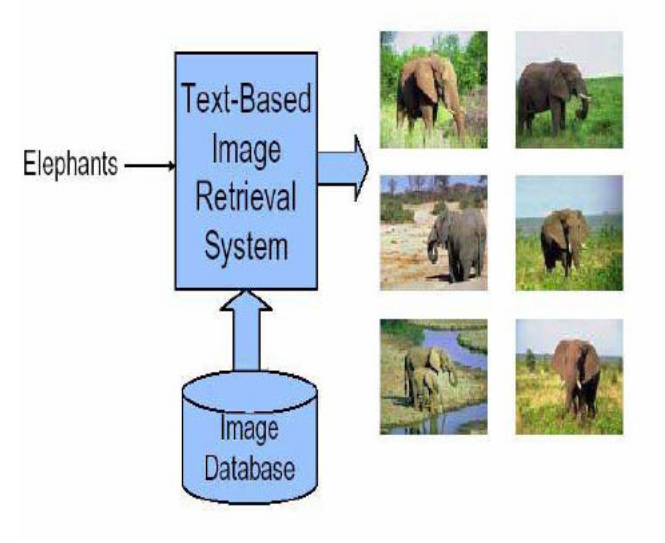
\includegraphics[width=3.5in]{Figures/textBasedIR.png}
	\caption[An Electron]{Recherche d'image par texte [Mee and Sus 13]}
	\label{fig:Electron}
\end{figure}

	Pour faire face à ce problème, d'autres techniques basées sur le contenu des images ont été développées, et qui font appel à deux domaines de recherches :

\textbf{Gestion de base de données:} Optimisation des méthodes de stockages, d'indexation multidimensionnel et du temps de réponse.

\textbf{Vision artificielle:} Représentation et extraction des caractéristiques des images.


\begin{figure}[H]
	\centering
		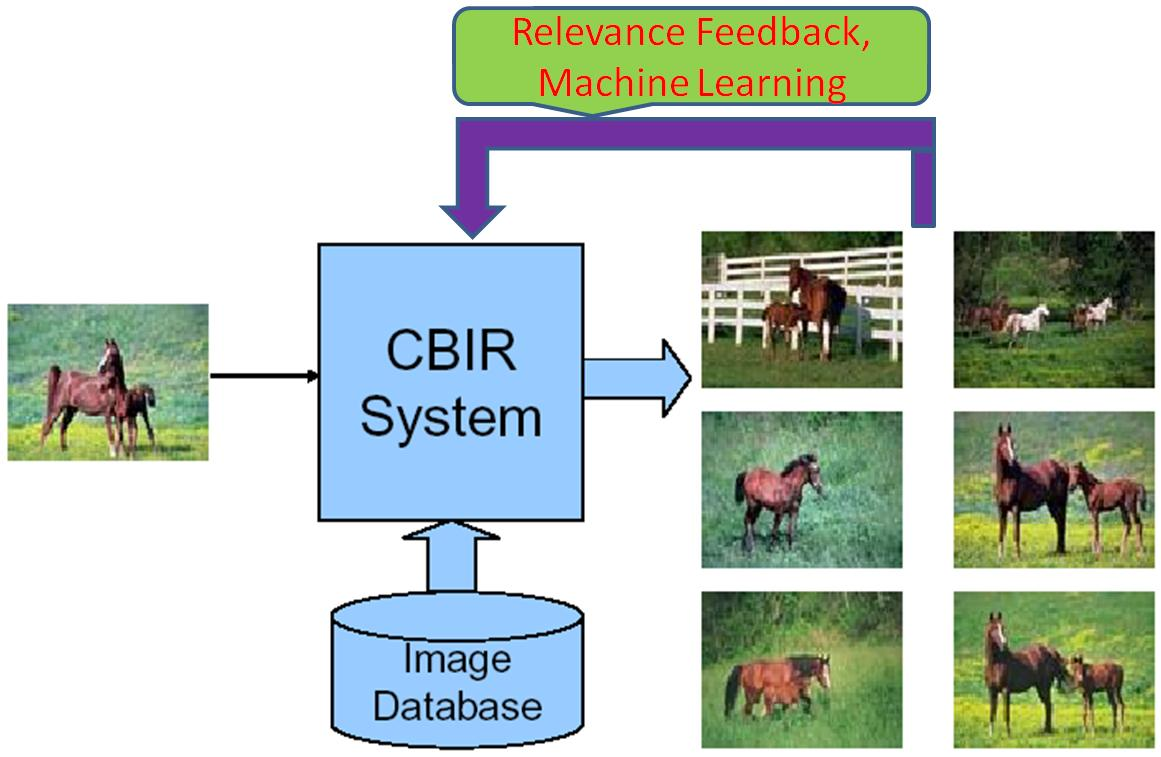
\includegraphics[width=3.5in]{Figures/cbir.JPG}
	\caption[An Electron]{Recherche d'image par le contenu [Mee and Sus 13]}
	\label{fig:Electron}
\end{figure}


\section{La conception d'un CBIR}

Les systèmes de recherches d'images par contenu sont généralement basés sur des caractéristiques prédéfinies qui sont:

\textbf{Descripteur  de couleur:} Grâce à  leurs représentations compactes et de faible complexité, la comparaison directe des histogrammes de couleur est communément utilisée.
\textbf{Descripteur de texture:} Matrice de co-occurence, Local Binary Pattern (LBP) [2]
\textbf{Descripteur de forme:} Descripteur de Fourier et moment invariants.
Et plus récemment, des descripteurs locaux tel que le SIFT sont utilisés.

\section{Calcule de similarité}
	Généralement, des fonction rigides de calcule de distance comme la distance euclidienne ou la similarité basée sur le cosinus sont utilisées pour la recherche de ressemblance entre les caractéristiques extraites.

	Par-contre, ces fonctions de calcul de distance et de similarité ne sont pas toujours optimaux pour la tache complexe de recherche par contenu sur des images, et ce du au problème du “gap sémantique” entre les caractéristiques bas niveau extraite par l'ordinateur et le haut niveau de perception humaine.

	De ce fait, récemment, de grand efforts ont été fournis dans la recherche de différentes méthodes de calcul de similarité en utilisant les techniques de l'apprentissage automatique.  Parmi ces dernières, des travaux se sont concentrés sur l'apprentissage de hachage ou code compacte. Des propositions ont été faites pour des méthodes d'apprentissage de MAPPING de données de hautes dimensions vers des codes binaires qui préservent la similarité sémantique.  [Sin and Ans 15]

\section{Types de CBIR}

	Quatre approches conceptuelles différentes ont été développées [Sin and Ans 15]:

\subsection{Basée-région :} Le Netra et Blobworld sont deux anciens systèmes de recherche d'images basés régions [6]. Pendant la recherche, un utilisateur est fourni avec des régions segmentées de l'image requête, et il est nécessaire d'attribuer plusieurs propriétés, telles que les régions à mettre en correspondance, les caractéristiques des régions, et même le poids des caractéristiques différentes [7].

\subsection{Basée-objets :} Les systèmes de récupération d'image basés sur les objets récupèrent des images à partir d'une base de données basée sur l'apparence des objets physiques dans ces images. Ces objets peuvent être des éléphants, des panneaux d'arrêt, des hélicoptères, des bâtiments, des visages, ou tout autre objet que l'utilisateur souhaite trouver. Une façon courante pour rechercher des objets dans les images est d'abord de segmenter l'image dans la base de données puis de comparer chaque région segmentée avec une région d'une certaine image requête présentée par l'utilisateur [8]. Ces systèmes de récupération d'image sont généralement couronnée de succès pour les objets qui peuvent être facilement séparés de l'arrière-plan et qui ont des couleurs distinctives ou des textures.

\subsection{Basée-exemples :} Nous nous intéresserons dans nos approches à cette catégorie qui sera détaillé dans le troisième chapitre. Les utilisateurs donnent une image d'échantillon, ou une partie d'une image, que le système utilise comme base pour le système recherche. Le système trouve ensuite les images qui sont semblables à l'image de base.

\subsection{Basée-Feedback :} Le système affiche l'utilisateur un échantillon de photos et demande à l'utilisateur des les classer. En utilisant ce classement, le système de ré-exécute les requêtes et répète cela jusqu'à ce que la bonne image soit trouvée.

\section{Systèmes et applications existants}


	Les techniques de CBIR ont été utilisées dans un grand nombre d'applications telles que: le diagnostic médical, les archives photographiques, l'identification des empreintes digitales, la reconnaissance faciale et les collections d'art.


\begin{figure}[H]
	\centering
		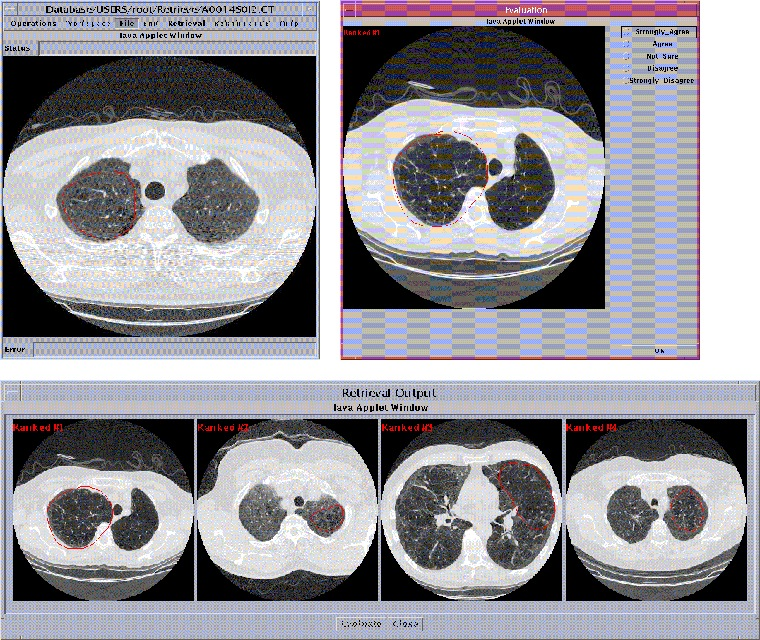
\includegraphics[width=3.5in]{Figures/cbirMedic.jpg}
	\caption[An Electron]{Application Médicale.}
	\label{fig:Electron}
\end{figure}


Fig 3. Application Médicale[4| Avinash]

Certains systèmes existants sont : 

\subsection*{QBIC}
	QBIC [6 | Niblack et tout] ou Query By Image Content, signifie requête par contenu d'image, il est le premier système de recherche d'images par le contenu commercial (CBIR). Il fournit des framework et des techniques de base pour de nombreux systèmes de récupération d'image. QBIC supporte les requêtes basée sur des exemples d'images, d'images construites par l'utilisateur et des dessins et modèles de couleur et de texture sélectionnés, etc. Les fonctions de couleur utilisées dans QBIC sont (R, G, B), (Y, i, q), ( L, a, b), et MTM (transformée mathématique Munsell), et un histogramme de couleur à k-élément. Dans son nouveau système, la recherche de texte par mot clé peut être combiné avec la recherche de similarité par contenu.



\subsection*{DigiKam}
	DigiKam est un logiciel gratuit et open-source organisateur d'image et éditeur de tag écrit en  C++. Il est une application de gestion de photos étendue construit avec des bibliothèques de KDE. Il offre, en plus de nombreuses autres fonctionnalités, les recherches inversées pour les images de la collection locale, la détection des doublons et une recherche floue par des dessins.

\subsection*{LIRE}
	LIRE est une bibliothèque Java qui fournit un moyen simple de récupérer des photos et des images en fonction de leurs caractéristiques de couleur et de texture. LIRE crée un index de Lucene des caractéristiques de l'image pour la récupération du contenu d'image basé (CBIR). Facile à utiliser, des méthodes pour rechercher l'index et les résultat sont fournies par LIRE. La bibliothèque LIRE et l'application de démo - ainsi que toutes les fichiers sources de test et de développement - sont disponibles sous la licence GNU GPL.

D'autres projets comprennent:
- The GNU Image-Finding Tool
- Google Image Search
- eBay Image Search

Une liste plus exhaustive peut être trouvée dans ce article :

$$https://en.wikipedia.org/wiki/List_of_CBIR_engines$$

\begin{figure}[H]
	\centering
		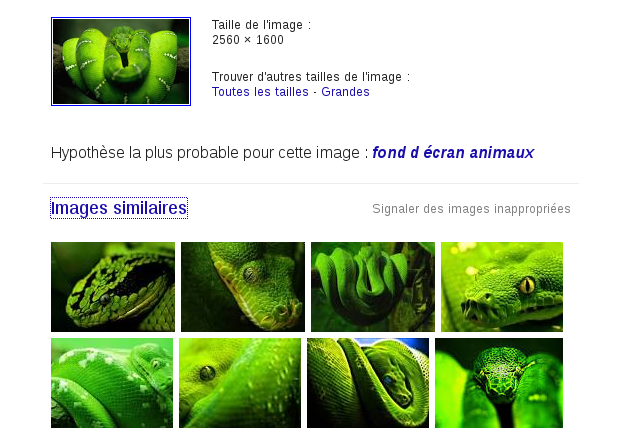
\includegraphics[width=3.5in]{Figures/googleImage2.png}
	\caption[An Electron]{Rechherche d'images de Google}
	\label{fig:Electron}
\end{figure}

\section{Problème du Semantic Gap}

	Parmi les problèmes  les plus difficiles qui font face au CBIR, nous trouvons le fossé sémantique. Il est défini comme la différence entre la faible niveau de représentation de l'information (y compris, mais pas seulement des images) dans l'ordinateur et la sémantique de haut niveau derrière elle (en d'autres mots, le sens qu'il est censé représenter).
Récemment, de nouvelles approches pour résoudre ce problème, consistent en appliquant des techniques d'apprentissage machine pour permettre à l'ordinateur de construire sa propre représentation hiérarchique d'une image au lieu de calculer les caractéristiques de manuellement.


\section{Conclusion}


%Chapter 2

\chapter{Apprentissage profond}

\section{Introduction}

	Quelles sont les limites de l'intelligence des ordinateurs? C'est une question toujours ouverte, même en étant l'une des toutes premières à être posées depuis l'invention des ordinateurs. Dans ce chapitre nous allons présenter l'une des techniques utilisées en intelligence artificielle qui est l'apprentissage automatique, Cette dernière permet d'ajouter à l'ordinateur la capacité d'apprendre et à s'adapter en fonction de la tâche qu'il doit accomplir.
	
	Nous aborderons ensuite l'une des techniques les plus récentes de l'apprentissage automatique qui est l'apprentissage profond (Deep Learning), elle propose une nouvelle approche plus approfondie et plus ressemblante au comportement du cerveau.


\section{Apprentissage automatique:}

	On peut trouver dans un dictionnaire que l'apprentissage est: "La capacité d'acquérir et d'appliquer les connaissances". C'est une notion que l'être humain a développé depuis son enfance, et si les ordinateurs arriveraient à développer la capacité d'apprendre?

	La tâche de l'apprentissage automatique est de concevoir un algorithme d'apprentissage fiable pouvant être utilisé pour résoudre différents problèmes et être appliqué dans différents domaines. Son utilisation pourrait couvrir plusieurs tâches très distinctes tel que la prévision du marché boursier, la découverte de caractéristiques et motifs dans les données scientifiques ou même la reconnaissance d'objets dans les images.

	En effet, à travers l'exploration du processus d'apprentissage du cerveau, les scientifiques ont fait l'hypothèse qu'il pourrait y avoir un algorithme d'apprentissage unique utilisé pour une variété de tâches. Cet algorithme unique pourrait donc à lui tout seul s'adapter à tous les problèmes qu'il rencontre. 

	Une expérience a été conçue en neuroscience au Département du MIT de Brain and Cognitive Sciences [Roe et al. 92], où ils ont coupé le lien entre l'oreille et le cortex auditif des furets, et y ont relié les nerfs optiques (Le cortex auditif étant la partie du cerveau responsable des processus qui traitent l'information auditive capturé par l'oreille). Ils ont découvert que le cortex auditif a pu apprendre à traiter les données optiques. En d'autres termes, la partie du cerveau qui une fois a appris à entendre, maintenant apprend à voir.

\begin{figure}[H]
	\centering
		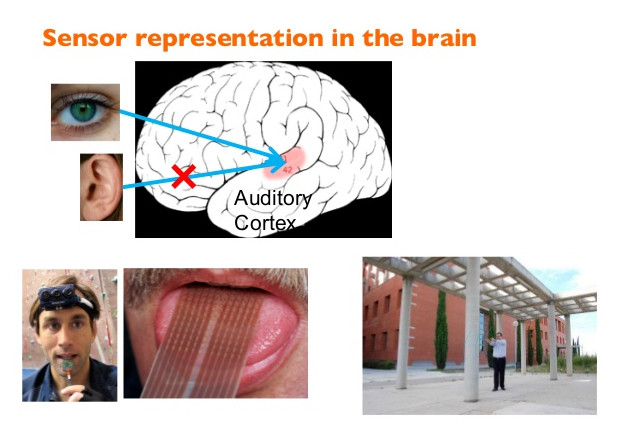
\includegraphics[width=5in]{Figures/OneLearningAlgoAndreNg.jpg}
	\caption[An Electron]{Représentation des sensations dans le cerveau.}
	\label{fig:Electron}
\end{figure}


	La même expérience a été reproduite avec succès à plusieurs reprises et avec des configurations différentes (différentes régions du cerveau, des espèces différentes, etc.) qui ont conduit aux mêmes résultats.

	L'apprentissage automatique vise à concevoir ce genre d'algorithme, un algorithme capable à s'adapter à toutes les situations possibles. L'objectif est de trouver des modèles dans les données utilisées pour l'apprentissage, et les généraliser pour construire des modèles mathématiques capables de faire des prédictions pour de nouvelles données.

\section{Concept de base de l'apprentissage:}


	D'après la définition de [Mit et al. 97] "Un programme informatique apprend d'une expérience \textit{E} à effectuer une tâche \textit{T} si sa performance \textit{P} mesurée pour cette tâche \textit{T} s'améliore avec l’expérience \textit{E}."

	La description des notions d'expérience, tâche et performance comme donné dans [Goo et al. 16] est très claire et peut être vue comme suit :

\subsection{Les tâches \textit{T}:} 
L'apprentissage automatique intervient dans des tâches où l'algorithmique classique est incapable de donner des résultats satisfaisants, ou prendrait simplement trop de temps. Ces tâches peuvent être par exemple des tâches de :

\textbf{Classification:} Où le programme doit trouver la classe $c \in C$ à laquelle une entrée \textit{X} appartient. En d'autres termes, on cherche à apprendre une fonction $F : \mathbb{R}^{n} \rightarrow C$ (C étant un ensemble discret ${1..k}$).

\textbf{Classification avec manque de données:} Elle rajoute un niveau de difficulté à la tâche de classification en supposant que certaines données peuvent être manquantes. Le classifieur devrait dans ce cas apprendre plusieurs fonctions avec différents sous ensembles des attributs de l'entrée \textit{X}.

\textbf{Régression:} Cette tâche ressemble à une classification, sauf que le résultat qui fut la classe devient une valeur numérique, et l'espace de sortie devient continu. Nous cherchons donc à trouver une fonction $F : \mathbb{R}^{n} \rightarrow \mathbb{R}$.

\textbf{Transcription:} Elle ressemble encore à la classification, sauf que ce que nous cherchons en sortie au lieu d’être une classe, est une séquence de symboles. Comme par exemple la traduction d'une phrase dans une autre langue.

\textbf{Détection d'anomalie:} Où le programme examine constamment une série d’événements ou de données d'entrée et signal s'il trouve quelque chose d'inhabituel. Une de ses applications est la détection de fraude dans l'utilisation de carte de crédit.

\textbf{Débruitage:} Permet d'apprendre à "nettoyer" une entrée \textit{x'} qui peut-être corrompue par un certain processus de corruption et retourner l'entrée originale \textit{x} .


\subsection{Les mesures de performance \textit{P}:}
La mesure de performance sert d'outil pour déterminer si un programme effectue bien la tâche \textit{T} souhaitée. La mesure diffère d'une tache à une autre. 

La mesure se fait sur les données dont ont dispose et qu'on utilise pour l'apprentissage, mais aussi sur une partie de données mise de coté (non utilisée pour l'apprentissage). Le plus important étant de savoir si le programme retournera de bons résultats sur des instances qu'il n'a jamais rencontré.   

Plusieurs mesures de performance existent pour les tâches de classification, la mesure de précision est généralement utilisée (nombre d'exemple bien classé sur le nombre total d'exemples). Mais pour d'autres tâches, le choix de la mesure peut être plus difficile à faire.

\subsection{L’expérience \textit{E}:}
L'expérience peut être définie par un scénario que le programme est sensé suivre durant son apprentissage, ce scénario est appelé un algorithme d'apprentissage.

Ces algorithmes se divisent en trois grandes catégories:
\textbf{Non-supervisé:} Le programme reçoit un ensemble de données (des exemples) qu'il se doit d'étudier pour satisfaire une tâche précise qui revient soit à minimiser un coût (pour augmenter la performance), soit à trouver des caractéristiques liants les attributs des exemples pour diviser ces derniers en catégories, par exemple: clustering, PCA, etc.

\textbf{Supervisé:} Le résultat du traitement de chaque exemple est connu. À chaque fois que le programme retourne la valeur de la fonction à apprendre, cette dernière est comparée avec la valeur juste (connue), si elle est conforme le programme est sur la bonne voie, sinon des modifications sur les paramètres appris doivent être effectuées.(ex: Réseaux de neurones, SVM, arbre de décision ... etc).

\textbf{Apprentissage par renforcement:} est un type différent des deux premiers dans le sens où le programme est perçu comme un agent qui interagie dans un environnement et qui reçoit des feedbacks lui permettant d’établir une "politique" qui vise à maximiser ses "gains" ou "récompenses", par exemple: Q-learning.


\subsection{Exemple d'algorithme d'apprentissage: Réseaux de neurones :}
Une des techniques les plus utilisées pour l'apprentissage automatique supervisé (et aussi pour le non-supervisé) est les réseaux de neurones (Perceptron multicouche). 
Un réseaux de neurones artificiel essaye d'imiter le fonctionnement des réseaux de neurones biologiques. Appelé aussi perceptron multicouche, ces derniers sont comme leur nom l'indique, formés de plusieurs couches de neurones. La première est la couche d'entrée, celles du milieu sont les couches cachées et la dernière est la couche de sortie.
Si on prend par exemple un réseau à une seule couche cachée:


\begin{figure}[H]
	\centering
		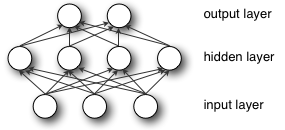
\includegraphics[width=3in]{Figures/mlp.png}
	\caption[An Electron]{Réseau de neurones à une seule couche cachée.}
	\label{fig:Electron}
\end{figure}

Chaque neurone prend en entrée un vecteur, le multiplie par un poids \textit{w}, et y rajoute un biais \textit{b}. Le résultat sera ensuite entré dans une fonction d'activation \textit{s} (qui peut être par exemple: $Sigmoide(x) = 1/(1+e^{x})$ ), et \textit{G} étant une fonction d'activation de la couche de sortie, cette dernière est choisie selon la tâche voulue (par exemple: regréssion, classification, etc.).
Tout le processus est schématisé par un calcul matriciel. L’expression de la fonction \textit{f} que nous essayerons d'apprendre serait :

$$f(x) = G( b^{(2)} + W^{(2)}( s( b^{(1)} + W^{(1)} x)))$$

Avec \textit{x} étant le vecteur d'entrée et \textit{w1}, \textit{ b1}, \textit{w2} et \textit{b2} étant les matrices de poids et vecteur biais entre respectivement, la couche d'entrée et la couche cachée, et entre la couche cachée et la couche de sortie. C'est ces paramètres qui seront appris.
Pour pouvoir se rapprocher de la fonction souhaitée, les paramètres à apprendre (\textit{w1}, \textit{ w2}, \textit{b1} et \textit{b2}) seront changés à chaque itération grâce à différents algorithmes, le plus utilisé étant l'algorithme rétropropagation du gradient (backward propagation of errors). 
Ayant le résultat souhaité et le résultat retourné, l'idée est de définir une fonction "coût" (l'inverse de la performance) qui décrira à quelle fonction \textit{f} serait-elle loin de ce qui est recherché. Ensuite dériver \textit{f} en fonction de chaque paramètre, et changer ces derniers dans le sens qu'il faut (rajouter à sa valeur, ou en soustraire).

Comme mentionné précédemment, l'apprentissage d'une tâche \textit{T} est sensé permettre une application de ce qui a été acquis sur de nouvelles données, ceci est appelé la généralisation.
La généralisation d'un apprentissage peut faire face à plusieurs problèmes, les plus majeurs sont:

\textbf{Le sur-apprentissage:} Quand le programme retourne de bon résultats sur les données d'apprentissage, mais n'arrive pas à généraliser sur des données qu'il n'a jamais rencontré auparavant.

\textbf{Le sous-apprentissage :} Dans le cas où le programme n'arrive même pas à trouver un modèle qui satisfait les données de l'apprentissage.


\begin{figure}[H]
	\centering
		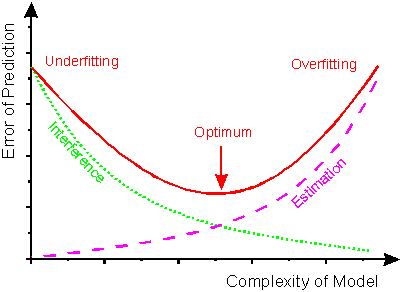
\includegraphics[width=3in]{Figures/image024.png}
	\caption[An Electron]{Sur-apprentissage et sous-apprentissage}
	\label{fig:Electron}
\end{figure}

\section{Introduction à l'apprentissage profond}

L'apprentissage profond est composé de deux mots: apprentissage et profond. La première partie réfère au fait que ce soit un concept d'apprentissage automatique, et la deuxième partie: profond, réfère à sa structure.

Principalement en raison de la faible puissance de calcul des machines, les algorithmes d'apprentissage n'étaient pas très complexes. Mais grâce à l'évolution exponentielle de la puissance de traitement (loi de Moore) de nouvelles perspectives ont été mises en lumière.
Depuis 2010, l'utilisation de la puissance des GPUs pour les calcules est devenue disponible pour le grand public, les scientifiques sont en mesure d'effectuer efficacement des calculs parallèles sur de très grosses matrices, et donc, ils ont réussi à élargir leurs modèles pour atteindre de manière significative de meilleures performances.


Le deep learning permet de développer des approches d'apprentissage automatique de plus en plus profondes (plus volumineuses et donc plus complexes) mais il permet aussi une très grande flexibilité pour combiner plusieurs techniques. Pourtant, beaucoup de problèmes restent à être réglés. Un des plus gros étant la soi-disant curse of dimentionality (la malédiction de la dimensionnalité). En fait, les données en entrée à un algorithme d'apprentissage sont de haute dimensionnalité. Une image par exemple, est une matrice de milliers, ou peut-être de millions de pixels, chacun peut prendre des centaines de valeurs différentes. Si nous prenons par exemple une image de $100 \times 100$, le nombre de configurations distinctes qu'elle peut prendre est:
$256^{3} \times 100 \times 100 = 1 677 721 600$.

Cet espace de valeurs est évidemment trop large pour pouvoir en couvrir même une fraction. Mais le problème serait plus à propos de fonctions de hautes variations que nous essayons de reproduire. En fait, si la fonction n'est pas trop complexe, même dans des dimensions élevées, quelques exemples pourraient être suffisants pour l'apprentissage de sa représentation, et si la fonction cible a beaucoup de variations, nous aurons besoin en conséquence de plusieurs exemples d'apprentissage, comme le montre la figure suivante:

\begin{figure}[H]
	\centering
		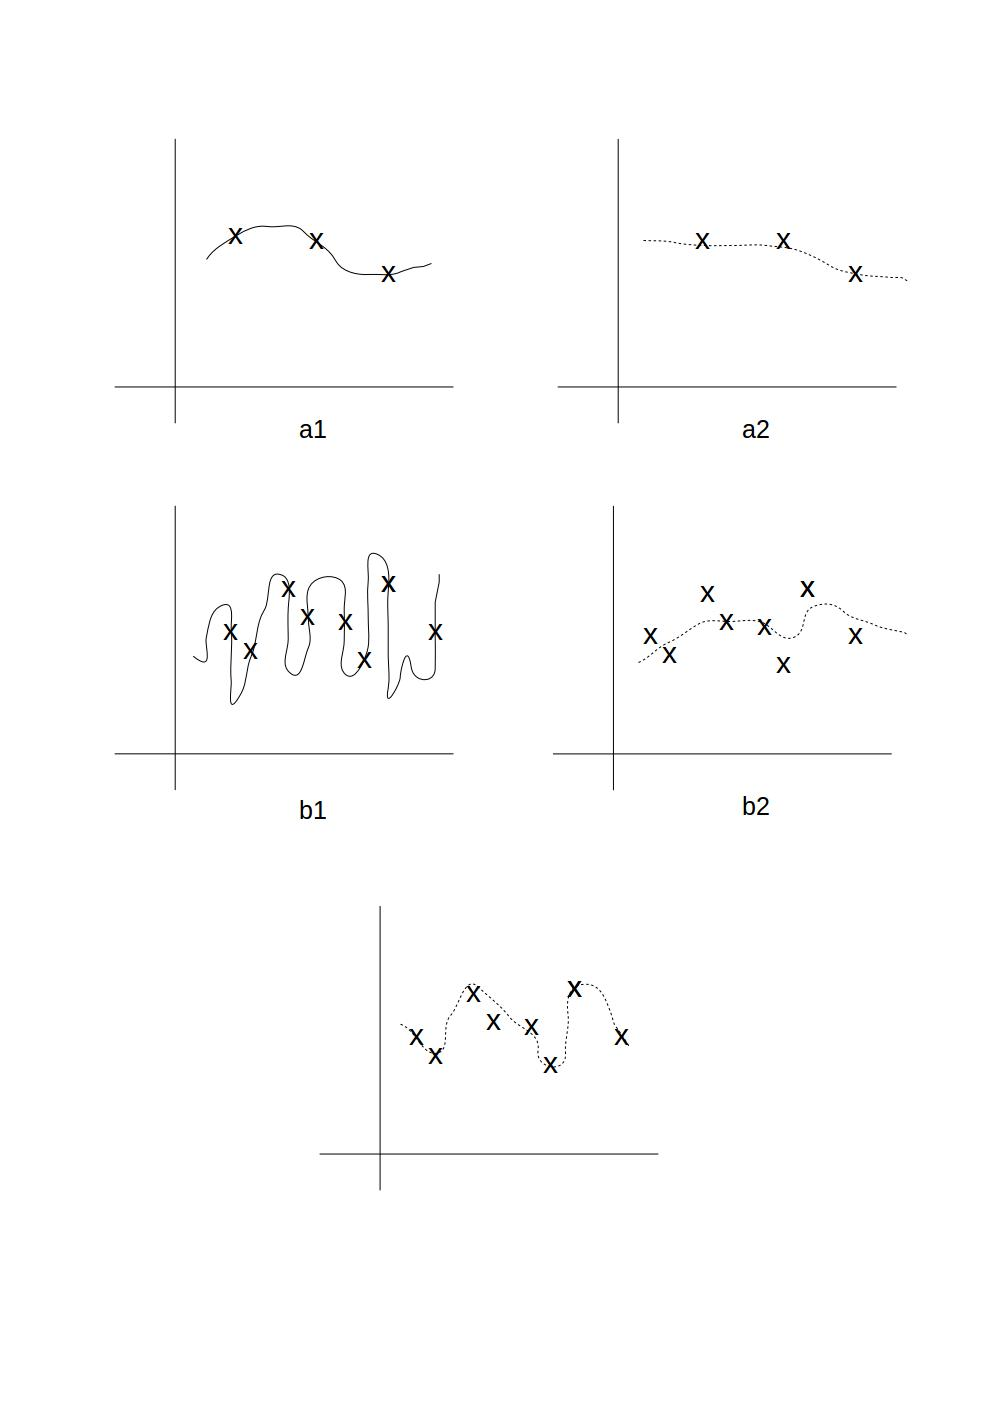
\includegraphics[width=3in]{Figures/highVariation.jpg}
	\caption[FA]{Fonctions d'approximation.}
	\label{fig:Electron}
\end{figure}


Dans l'exemple 1, le graphe (a1) montre une fonction simple que le modèle cherche à approximer, et le graphe (a2) montre le résultat de l'approximation obtenu par le modèle. Ce résultat est satisfaisant malgré le nombre  réduit d'exemples.

Quant à l'exemple 2, le graphe (b1) montre une fonction plus complèxe que celle du graphe (a1), la tâche d'approximation devient plus difficile. Les tentatives du modèle  (représentées respectivement par les graphes (b2) et (b3)) de ne pas passer par tous les exemples, ou de passer par tous les exemples échouent à trouver un résultat satisfaisant dans les deux cas. 

Pour une dimension \textit{D} de donnée en entrée (exemple: age, sexe, etc.) ou sur une variété de dimension D, le nombre de variations peut croître de façon exponentielle avec \textit{D}, d'où résulte le grand nombre d'exemples requis. [Yos 14]

\section{Les Architectures de l'apprentissage profond:}

Bien que le principe des algorithmes d'apprentissage existants est unique (en passant par un tas de données pour trouver des modèles significatifs et construire des modèles mathématiques afin de réaliser une tâche d'apprentissage), pour s'adapter à des objectifs différents, plusieurs concepts et architectures sont appliqués, parmi eux:
 

\subsection{Deep Belief Networks}

Réseaux profond de croyance est une pile de machines de Boltzmann restreintes (RBM) qui se termine généralement avec une unité de classification. Un RBM est un réseaux de neurones à deux-couches (une visible et l'autre cachée) stochastique (l'activation de neurones est probabiliste)

Les DBN sont utilisés pour le pré-apprentissage non-supervisé, pour une meilleure initialisation des poids.



\subsection{Réseau de neurones à convolution}
L'idée a été inspirée du travail de Hubel et Wesley sur le cortex visuelle du chat [Hub et al. 68]. Un réseau de neurones à convolution ou Convolutional Neural Network (ConvNets), vise à émuler le réseau de neurones biologique.
	La mise en œuvre la plus commune d'un réseau de neurones à convolutions est LeNet de [Lec and Wie 98], qui empile différentes couches de convolution et sous-échantillonnage, suivies à la fin d'une multicouche de perceptrons entièrement connectés comme indiqué sur la figure suivante :

\begin{figure}[H]
	\centering
		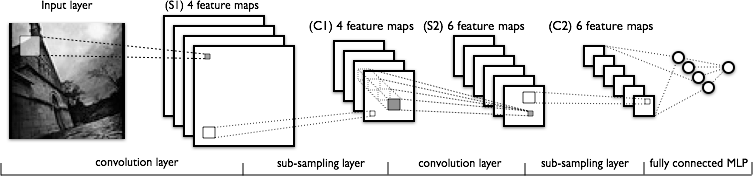
\includegraphics[width=5in]{Figures/Mylenet.png}
	\caption[An Electron]{Exemple de couches de convolution.}
	\label{fig:Electron}
\end{figure}


\subsubsection{La convolution}
La convolution est un terme mathématique, définie comme l'application d'une fonction de façon répétée à travers la sortie d'une autre fonction. Dans ce contexte, il signifie d'appliquer un filtre sur une image en prenant en compte tous les décalages possibles. Comme le montre la figure suivante:


\begin{figure}[H]
	\centering
		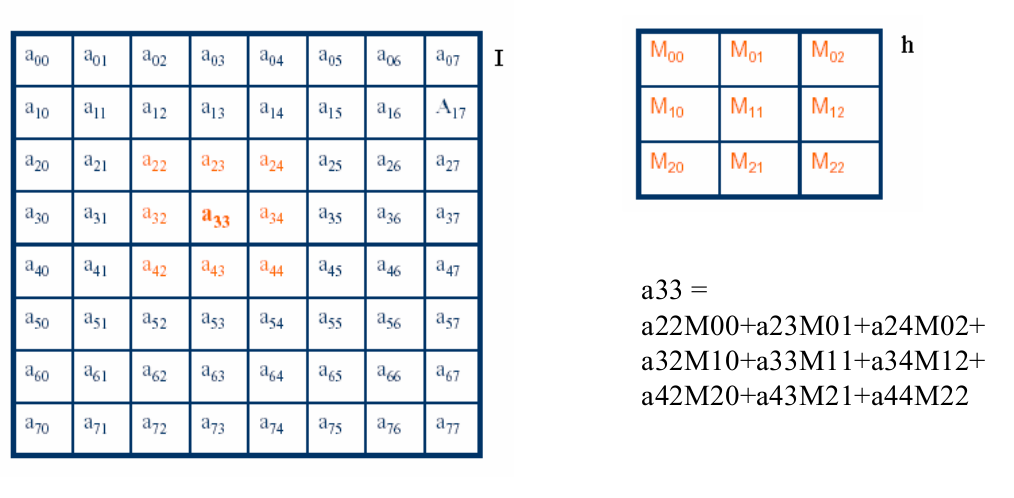
\includegraphics[width=5in]{Figures/convAouat.png}
	\caption[An Electron]{Exemple de convolution}
	\label{fig:Electron}
\end{figure}



Les couches de convolution appliquent simplement des convolutions sur les couches précédentes en utilisant différents filtres. Les poids de chaque filtre sont appris grâce à une rétropropagation (backpropagation).

\subsubsection{Le padding}
Afin de mieux contrôler la taille des images obtenues après l'application d'une convolution sur une image en entrée, on peut utiliser ce qu'on appelle "padding" (remplissage) avant une convolution.
L'une des techniques utilisée pour le padding est le zero-padding, pour cela il suffit de rajouter des zéros aux bords de l'image. Pour un zero-padding de 1, on a le résultat de la figure suivante:

\begin{figure}[H]
	\centering
		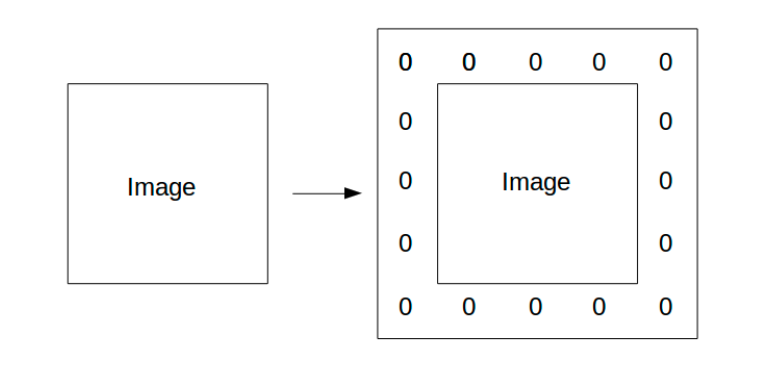
\includegraphics[width=5in]{Figures/zero-padding.png}
	\caption[An Electron]{Application d'un zero-padding sur une image}
	\label{fig:Electron}
\end{figure}

Nous pouvons aussi utiliser le zero-padding pour conserver exactement la taille spatiale d'une image après l'application d'une convolution, de sorte que la largeur d' entrée et de sortie et la longueur sont les mêmes, comme nous le verrons dans le prochain chapitre.


\subsubsection{Le sous-échantillonnage}
Le sous-échantillonnage (ou subsampling) se réfère à la réduction de la taille globale d'un signal. Dans de nombreux cas, comme la compression audio pour les fichiers de musique, le sous-échantillonnage se fait simplement pour la réduction de la taille. 

La méthode de sous-échantillonnage spécifique utilisée dans LeNets est connue comme max-pooling. Cela implique le fractionnement d'une matrice (image) en de petits fragments qui ne se chevauchent pas (plus les fragments sont grands, plus la réduction est importante), et de prendre la valeur maximale dans chaque grille en tant que la valeur dans la matrice réduite. 
Ceci permet, entre autre, l'obtention d'une invariance aux translations. La figure suivante montre un exemple de l'application d'un max-pooling:


\begin{figure}[H]
	\centering
		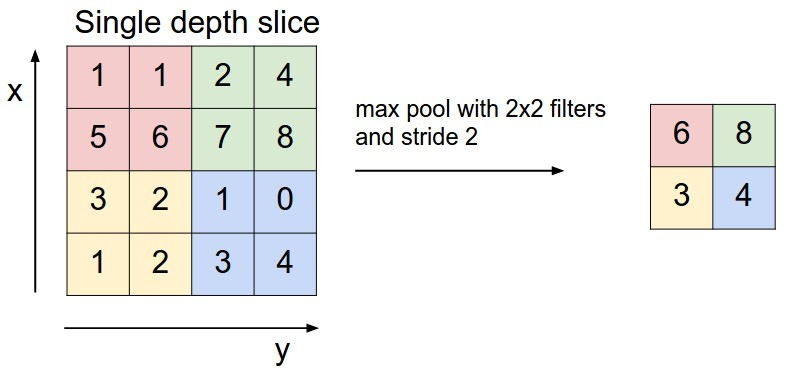
\includegraphics[width=5in]{Figures/maxpool.jpeg}
	\caption[MP]{Exemple max-pooling}
	\label{fig:Electron}
\end{figure}

\subsubsection{Normalisation}
Une des techniques inspirée de la neuroscience computationnelle qui a été utilisée, est l'ajout de couches de normalisation après une couches de convolution. [Kri et al.,12] Néanmoins, la normalisation il semble que ces couches ont un impact très minime et ne sont plus utilisées. Ils ont été dominé par d'autres techniques tels que le "dropout" ainsi qu'une meilleure initialisation des poids des neurones et les algorithmes d'entraînement du réseau.

\subsubsection{Perceptron multicouche entièrement connecté:}

Finalement, après plusieurs couches de mise en commun de convolution et de max-pooling, le traitement final dans le ConvNets se fait via des couches de perceptrons entièrement connectés. Une couche entièrement connectée prend tous les neurones de la couche précédente et les relies à chaque neurone dont elle dispose.

\subsubsection{Dropout}
On applique un dropout lors de la phase d'entraînement d'un réseau de perceptron  multicouche entièrement connecté, précisément lors de la rétropropagation. Son est d'éviter le sur-apprentissage, par exemple pour un taux de dropout de 30\%, la rétropropagation ne s'appliquera pas sur 30\% des neurones d'une couche (ces neurones sont choisis aléatoirement à chaque rétropropagation). Dans ce cas les neurones d'une même couche n'auront pas rencontré (n'apprendront pas) les même exemples (images).

\subsection{Deep Auto-encoders}

Nous avons déjà parlé du problème de curse of dimentionality. Les Autoencoders sont un moyen de résoudre ce problème. Pour cela, ils visent à trouver une représentation compressée des données en entrée.
En d'autres termes, les autoencoders sont un type de réseaux de neurones entraînés d'une manière supervisée par rétropropagation pour reproduire leurs données en entrée après les avoir fait passées à travers des couches cachées de dimension inférieure à celle de l'entrée.

%Une des techniques pour former un "deep autoencoder" de empilant pré-entraîné, et d'ensuite faire une mise au point à la fin avec de la rétropropagation.

Un "deep autoencoder" est construit en empilant un certain nombre de couches de machines de Boltzmann restreintes RBM pré-entraîné. On applique à la fin sur ces couches une mise au point (fine tuning) avec de la rétropropagation (backprop).

Un exemple d'utilisation d'un autoencoder est la recherche d'une représentation de dimension inférieure pour une image. La raison pour laquelle cette représentation pourrait exister est donnée par l'idée suivante :
Si vous essayez de générer une image aléatoire, vous vous  retrouverez très probablement avec une image comme le montre la figure suivante. Peu importe combien de fois vous essayez, vous obtiendrez probablement jamais une image d'un chien, d'une voiture, ou autre chose significative.


\begin{figure}[H]
	\centering
		
\includegraphics[width=3in]{Figures/randomImageGEn.JPG}
	\caption[An Electron]{Image générée aléatoirement.}
	\label{fig:Electron}
\end{figure}

Ainsi, l'espace des images significatives forme seulement une fraction de l'espace total défini par les valeurs des pixels. L'objectif de l'autoencoder est alors de trouver une représentation d'une image dans cet espace.


\begin{figure}[H]
	\centering
		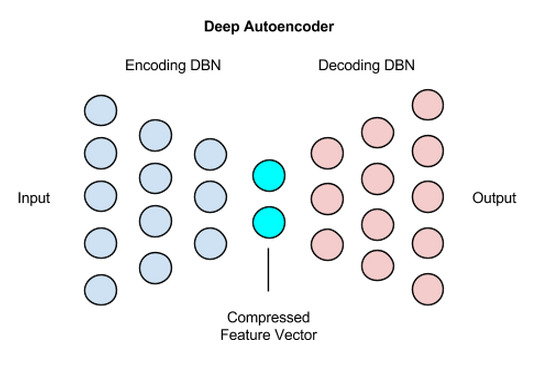
\includegraphics[width=3in]{Figures/deep_autoencoder.png}
	\caption[An Electron]{Exemple d'un modèle d'autoencoder utilisant les DBN.[Site2]}
	\label{fig:Electron}
\end{figure}

\section{Les exploits des techniques d'apprentissage profond [Jia 14]}

L'Apprentissage profond a surperformé les techniques de vision artificielle traditionnelles au cours des dernières années. Dans le concours ImageNet en 2010 (ImageNet est un projet qui a pour but de fournir aux chercheurs une très grande base d'images facilement accessible), le meilleur algorithme de Vision artificielle traditionnelle avait un taux d'erreur de 28,2\%, ce qui signifie qu'il a obtenu de 71.8\% d'images correctes. En 2011, le meilleur algorithme à obtenu un taux d'erreur de 25,8\%. 

	En 2012, cependant, le premier processus d'apprentissage profond est entré dans la compétition et a dépassé en performance toutes les méthodes traditionnelles avec un taux d'erreur de 16,4\%. 
	Après cela, le premier algorithme d'apprentissage profond a ouvert les portes, la compétition a été inondée avec d'autres équipes d'apprentissage profond qui ont atteint un taux d'erreur de 11,7\% en 2013 et 6,7\% en 2014 \textbf{MACHI 7.405\% imagenet website agrees ???? Chap 3}. Le vainqueur de l'édition 2014 a reconnu 93\% des images, un énorme bond en avant surtout par rapport au taux de 72\% atteint par les techniques de vision artificielle traditionnelles en 2010.


\begin{figure}[H]
	\centering
		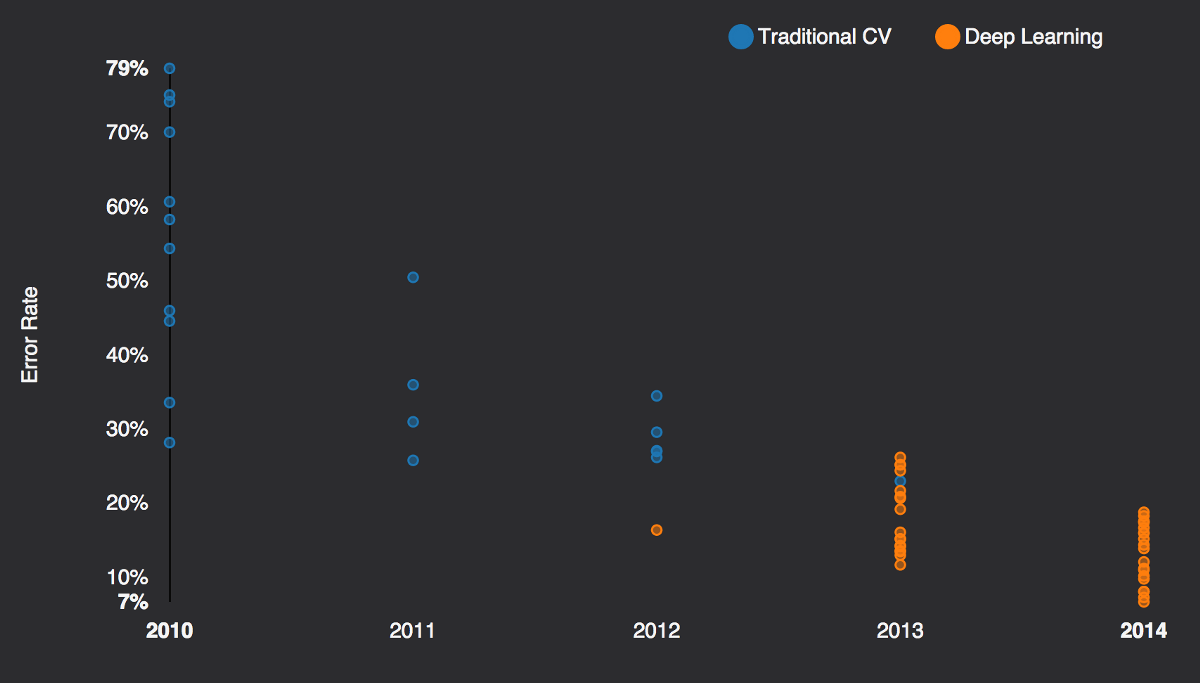
\includegraphics[width=5in]{Figures/clairifaiIMAGENET.png}
	\caption[An Electron]{Résultats du concours d'IMAGEnet.}
	\label{fig:Electron}
\end{figure}


\section{Conclusion}


 
%Chapter 3

\chapter{Recherche sémantique d'images} % Main chapter title

\section{Introduction}
	Dans ce chapitre nous allons présenter nos différentes approches pour la réalisation d'une recherche d'image par le contenu (CBIR) basée exemple. Contrairement aux techniques traditionnelles qui utilisent les formes, textures, couleurs, etc. pour comparer les images (calculer la ressemblance), nous allons utiliser dans nos approches des techniques de l'apprentissage profond. Parmi ces techniques nous allons nous intéresser aux réseaux à convolution (ConvNets) et aux Deep AutoEncoders.

Nous allons aussi faire un effort pour donner des interprétations bien fondées des différents résultats que nous allons obtenir grâce aux méthodes d'apprentissage.

\section{Recherche d'image par le contenu basée exemple}
	Parmi les types de la recherche d'image par le contenu mentionnées au chapitre 1, nous avons choisi celle basée exemple pour sa facilité d'implémentation. Afin de comparer nos différentes approches, nous allons calculer pour chacune les mesures de performance obtenues. Pour cela nous allons appliquer notre algorithme de recherche d'image par le contenu basée exemple comme suit:

\begin{algorithme}
\caption{Recherche d'images par le contenu basée exemple}
\Function{CBIR}
{\textit{Base}: \textbf{Base d'images}, \textit{Comp}: \textbf{Approche de Comparaison}}{Mesures de performance}
{
\begin{enumerate}


\item Diviser \textit{Base} en deux parties:
\begin{enumerate}[a]
\item \textit{Query}: Extraire aléatoirement de chaque classe de \textit{Base} 20\% d'images.
\item \textit{Test}: Les 80\% restantes.
\end{enumerate}

\item \For {chaque classe \textit{C} de \textit{Query}}
{
\begin{enumerate}
\item \For {chaque image $\textit{Q}\in\textit{C}$ de \textit{Query}}
{
	\begin{enumerate}[a]
	\item \For {chaque image \textit{T} de \textit{Test}}
	{
		Calculer la ressemblance \textit{R} entre \textit{Q} et \textit{T} avec l'approche 
		
		\textit{Comp}.
	}
	\item \textit{Resemb} = liste des images de \textit{Test} triées selon \textit{R} par ordre 
	
	
	décroissant.
	\item Comparer la classe \textit{C} de \textit{Q} avec les classes des images 
	
	triées \textit{Resemb}
	\item Calculer les mesures de performance \textit{Perf}.
	\end{enumerate}
}
\item Calculer la moyenne des mesures de performance de \textit{C}.
\end{enumerate}
}
\item Retourner la moyenne des mesures de performance Totale.
\end{enumerate}
}
\end{algorithme}

	La recherche d'image par le contenu basée exemple nécessite une grande base d'image, pour cela nous avons utilisé deux bases différentes, la première est celle de WANG [Wan et al.,01][Li et Wan.,03] contenant 1000 images (10 classes de 100 images), et la deuxième est Caltech101 (100 classes) [Fei et al. 04] contenant plus de 9000 images. Nous avons choisi ces deux bases d'images pour la simple raison qui est que les images sont déjà classées (une classe unique pour une image), ce qui facilitera le calcul des mesures de performance.
	
	La première étape de notre algorithme est de diviser une base contenant plusieurs images en deux parties: Nous appellerons la première \textit{Query}, contenant 20\% des images (choisies aléatoirement) qui seront utilisées en tant que requêtes. Les 80\% des images restantes seront dans la deuxième partie que nous appellerons \textit{Test}.

	Notre but étant que pour chaque image requête de \textit{Query}, nous allons trouver les images qui lui ressemblent le plus de la partie \textit{Test}. Nos méthodes de comparaison (calcul de ressemblance) entre les images ce feront avec plusieurs approches \textbf{que nous allons présenter plus bas}.

	En ayant la liste des images les plus ressemblantes à une requête donnée triée par ordre décroissant (de l'image la plus ressemblante à la moins ressemblante), et pour comparer nos différentes approches que nous avons réalisé, nous devons calculer les mesures de performance qui sont comme suit : 
\begin{enumerate}

\item Précision à 1: 1-Précision, elle est égale à 100\% si l'image la plus ressemblante à la requête qui est retournée par l'approche est effectivement de la même classe que l'image en entrée, et 0\% dans le cas contraire.
\item Précision à \textit{N}: ou N-Précision \textit{N} étant un nombre d'images (5,10,20,40 ou 60). Cette mesure donne le pourcentage d'images qui appartiennent à la même classe que l'image requête, parmi les \textit{N} images les plus ressemblantes.
\item Rappel: C'est le pourcentage d'images qui sont de la même classe que l'image requête, parmi le nombre de toutes images qui appartiennent réellement à cette classe.
\item Taux d'erreur: C'est l’événement contraire de la 1-Précision.

%$$ N-précision = \dfrac{images réelement pertinentes top-N}{N} Rappel = \dfrac{Img Per}{N}$$

\end{enumerate}

	Contrairement à la base d'images WANG, nous avons remarqué que les classes de la base Caltech101 (101 classes) ont un nombre d'images qui est différent entre chaque classe, nous allons donc d'abord calculer les moyennes de performance d'une classe donnée, ensuite calculer la moyenne des performances totale de l'approche. Comme ça les classes ayant un nombre très grands (très petits) d'images, ne seront pas plus avantagées (moins avantagées) par rapport aux autres classes.
	
\section{Architecture du réseau à convolution}
	Comme nous l'avons cité précédemment, notre approche utilisera des techniques d'apprentissage profond pour la comparaison des images à la places des techniques traditionnelles (texture, forme, couleur, etc.). Pour cela, nous avons utilisé les réseaux à convolution (ConvNets) introduits dans le chapitre précédent.
	
	L'architecture VGG-CNN-S du réseau à convolution que nous avons utilisé dans notre algorithme, a été proposée par l'équipe de recherche Visual Geometry Group Department of Engineering Science, Université d'Oxford (VGG) [Cha et al.14]. Lors de la compétition ImageNet 2014 (introduite au chapitre 2) ils ont pu obtenir une erreur de classification (top-5) de 7.405\%. L'architecture VGG-CNN-S du ConvNets a été entraîné sur une base d'image très grande ILSVRC-2012 (plus de 1.2 millions d'images [Rus et al.15]). Cette base contient 1000 classes différentes, elle inclue une très grande variété d'images et a donc beaucoup de potentiel pour être généralisable, c’est-à-dire elle peut donner aussi de bons résultats sur d'autres bases d'images qui sont plus petites que celle ILSVRC-2012.
	
	Nous allons donc commencer par décrire l'architecture VGG-CNN-S du réseau à convolution que nous avons utilisée. Le tableau ci-dessous donne une descriptions de chacune des couches de l'architecture du ConvNets utilisé qui est comme suit:

\begin{figure}[H]
\begin{center}
\begin{tabular}{|c|c|c|c|c|c|c|c|}
  \hline
96x7x7 & 256x5x5 & 512x3x3 & 512x3x3 & 512x3x3 & 4096 & 4096 & 1000\\
st. 2, pad 0 & st. 1, pad 1 & st. 1, pad 1 & st. 1, pad 1 & st. 1, pad 1 & drop- & drop- & soft-\\
LRN, x3 pool & x2 pool & - & - & x3 pool & out & out & max\\
  \hline
\end{tabular}
\end{center}
\caption{Architecture de VGG-CNN-S [Cha et al.14].}
\end{figure}
	Ce réseau à convolution comporte une couche d'entrée (non incluse dans le tableau), 7 couches cachées et une couche de sortie (la dernière colonne du tableau). Les données en entrée au réseau à convolution sont des images ayant une taille fixe de 224 x 224 pixels RGB. Si l'image en entrée a une dimension plus grande, elle devra être redimensionnée en 224x244 pixels, en gardant la partie centrale de l'image. Le choix de la valeur de 224 pixels est nécessaire pour que les données en entrée s'adaptent à l'architecture proposée. Le seul pré-traitement effectué est la soustraction de la valeur moyenne RGB de chaque pixel de l'image, son interprétation géométrique est de centrer le nuage de donnée autours d'une origine [CS231n 16].

	L'image passe premièrement à travers des piles de couches de convolution où nous appliquons plusieurs filtres. La première couche de convolution applique 96 filtres différents de taille $7x7$ pixels avec un stride de 2 et sans zero-padding, comme le montre la figure suivante:

\begin{figure}[H]
	\centering
		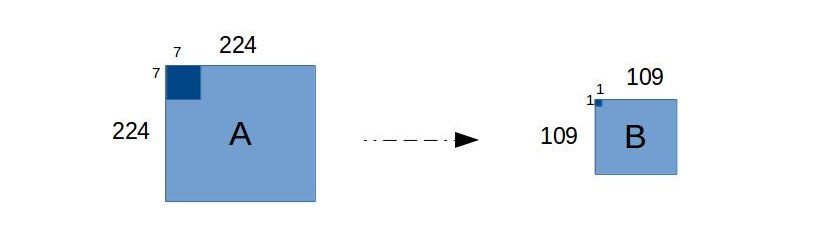
\includegraphics[width=5in]{Figures/conv.jpg}
	\caption[An Electron]{Application d'un filtre de convolution.}
	\label{fig:Electron}
\end{figure}

	La valeur du stride représente le nombre de pixels de déplacement d'un filtre sur une image après chaque opération de convolution. Le passage d'une image à travers une pile de convolution aura pour effet de changer la dimension (nombre de pixels) de l'image. Posons $S$ la valeur du stride, $P$ la valeur du zero-padding, $W_{1}$ le nombre de pixels d'une dimension (longueur ou bien largeur) d'une image et $F$ la taille des filtres de convolution. Pour calculer la taille obtenue en sortie $W_{2}$, on applique la formule suivante:
$$W_{2} = (W_{1} - F + 2*P)/S + 1$$
$$Exemple de la première convolution: (224 - 7 + 2*0)/1 +1 = 109.5$$
	
	Si on obtient un nombre non entier (avec une virgule) comme l'exemple ci-dessus, ce qui représente une opération de convolution incomplète, on prend donc que la partie entière. Comme les images en entrée ont la même largeur et longueur (images carrées), il suffit seulement de calculer cette valeur (nouvelle dimension) pour une seule dimension.
	Cette première couche de convolution est la seule couche sur laquelle on applique une normalisation [Kri et al.,12]. Après cela, on applique un max-pooling sur la sortie résultante des convolutions, comme le montre la figure suivante:

\begin{figure}[H]
	\centering
		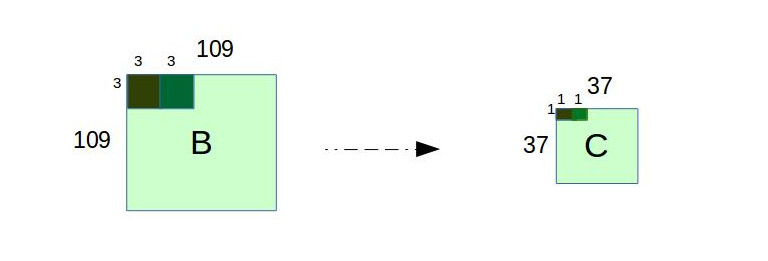
\includegraphics[width=5in]{Figures/pool.jpg}
	\caption[An Electron]{Application d'un max-pooling.}
	\label{fig:Electron}
\end{figure}

	En posant $W_{1}$ le nombre de pixels d'une dimension d'une image, $F$ la taille du max-pooling et $S$ la valeur du stride qui est égale à $F$. On peut calculer la taille du résultat $W_{2}$, comme suit:

$$W_{2} = (W_{1} - F )/S + 1$$
$$Exemple du premier max-pooling: (109 - 3)/3 +1 = 36.33$$

	Ces étapes sont presque les mêmes pour chaque couche de convolution, chacune applique des filtres de convolution d'une certaine taille, suivi ou non d'un max-pooling. On remarque sur la figure qui va suivre dans la troisième couche de convolution, que la taille de l'entrée est de 17x17 et de la sortie 17x17, comme on a dit dans le chapitre précédent cela est dû au zero-padding qui permet de contrôler la dimension des sorties. On remarque aussi que la plus petite taille des filtres de convolution est de 3x3 pixels, et cela pour capturer la notion de gauche / droite, haut / bas, au centre.

	Les sorties obtenues après le passage d'une image sur ces couches de convolutions sont 512 matrices de taille 6x6 pixels, 512 étant le nombre de filtres appliqués lors de la dernière convolution, et la taille 6x6 pixels est la taille de la sortie de cette même couche après application des filtres de convolution et du max-pooling.

	L'empilement des couches de convolution est suivi par trois couches (les 3 dernières couches du tableau) entièrement connectées (Fully-Connected Layers), pour faire passer en entrée les valeurs des sorties des convolutions on devra aplatir les matrices obtenues précédemment (521 matrices de 6x6 pixels) en un vecteur unidimensionnel, comme le montre la figure suivante:

\begin{figure}[H]
	\centering
		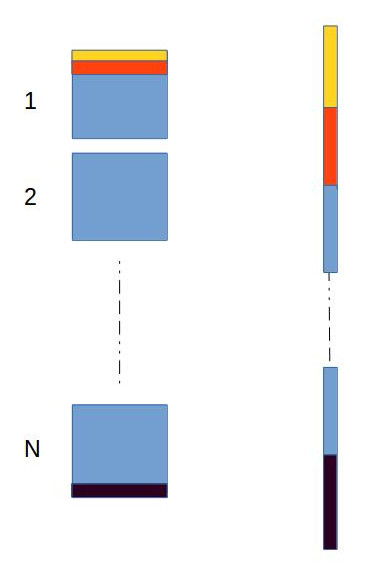
\includegraphics[width=2.5in]{Figures/flattening.jpg}
	\caption[An Electron]{Applatissement des résultats du ConvNets.}
	\label{fig:Electron}
\end{figure}

	Le vecteur unidimensionnel sera composé de la succession des lignes de la première matrice, ensuite les lignes de la deuxième matrice, et ainsi de suite jusqu'à la dernière matrice. Donc dans notre cas, à partir de 512 matrices de 6x6 nous aurons un vecteur unidimensionnel de taille: $512*6*6 = 18432$.

Les deux premières couches entièrement connectées ont 4096 neurones chacune, la troisième et dernière couche du réseau est la couche soft-max. Elle réalise la classification de la base d'image ILSVRC-2012 et contient donc 1000 neurones (un pour chaque classe), cette couche soft-max donnera comme sortie un vecteur de 1000 valeurs contenant les probabilités d'appartenance d'une image aux 1000 classes.

	La figure suivante montre l'architecture complète contenant la taille de chaque entrée et sortie de chaque couche du réseau à convolution:

\begin{figure}[H]
	\centering
		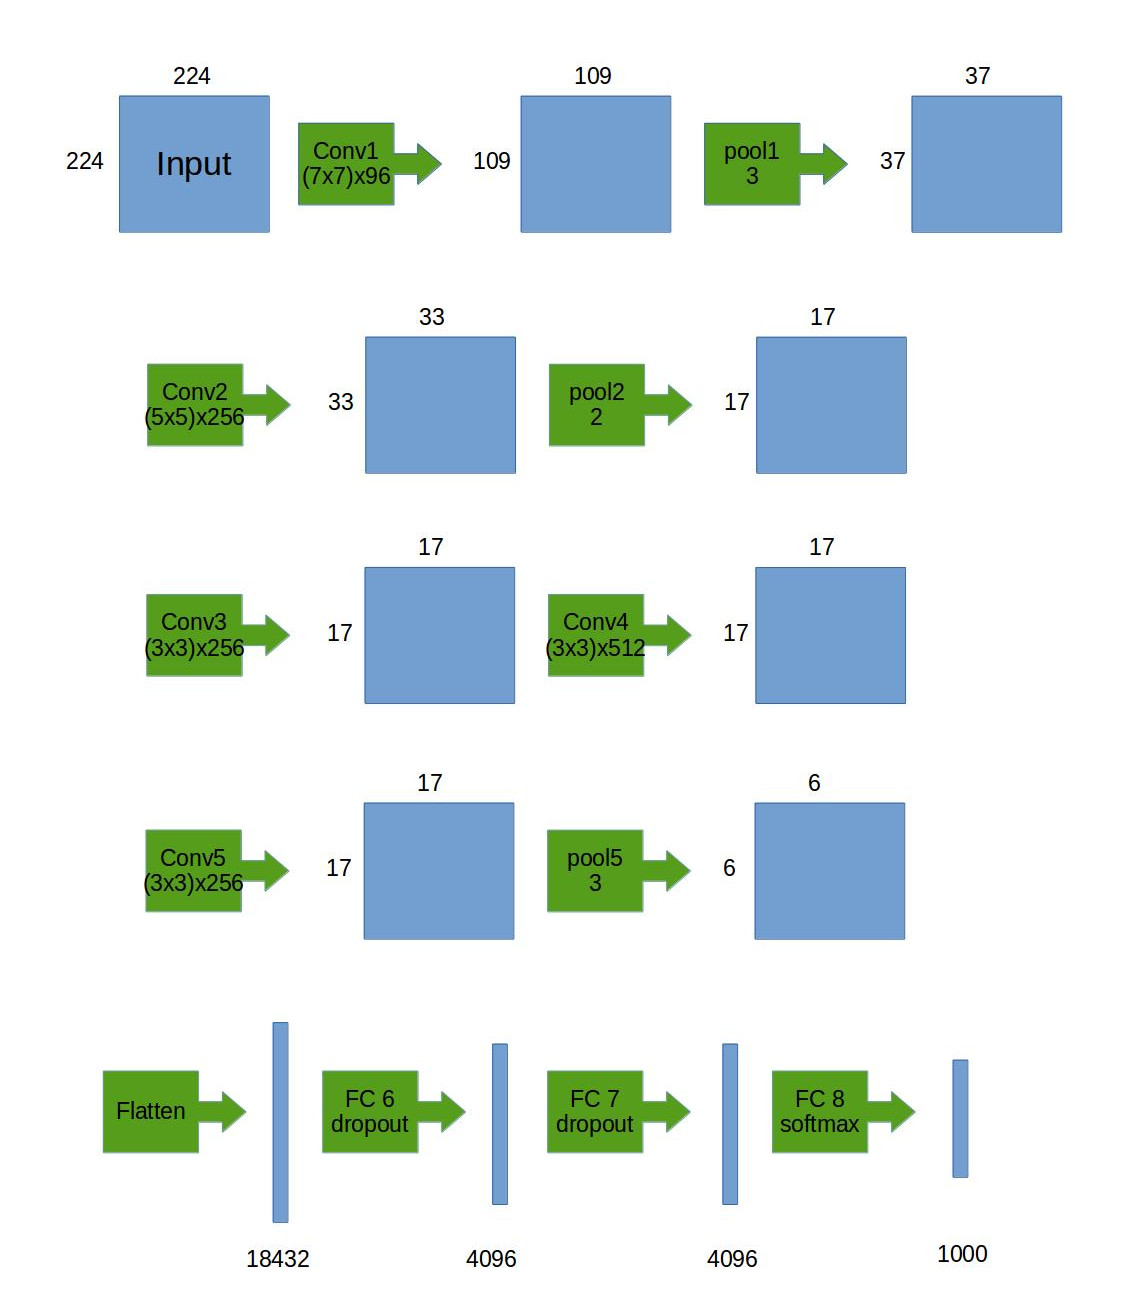
\includegraphics[width=6in]{Figures/architectureVGG.jpg}
	\caption[An Electron]{Architecture complète du ConvNets.}
	\label{fig:Electron}
\end{figure}



\section{Entraînement du réseau}
	Comme pour un réseau de neurones ordinaire, un réseau de neurones à convolution a besoin d'être entraîné sur une base d'exemple (base d'images dans notre cas), plus le réseau a une grande taille (plusieurs poids) plus on aura besoin d'un plus grand nombre d'exemples pour son entraînement. 
	
	La base utilisée pour l’entraînement (apprentissage) de ce réseau à convolution est ILSVRC-2012 (plus de 1.2 million d'images), et l'apprentissage s'est fait avec une descente du gradient stochastique avec moment. Les paramètre empiriques (hyper-paramètres) sont comme suit: Un moment de $0.9$, une dégradation des pondérations (weight decay) $de 5*10^{-4}$, et un taux d'apprentissage initial (learning rate) de $10^{-2}$. [Cha et al.14]
	
	Les valeurs initiales des poids ne peuvent pas être toutes égales à zéro (ou une autre valeur), puisque tous les poids vont calculer le même gradient lors de la rétro-propagation, ce qui résultera en l'application des mêmes mis-à-jours sur tous les poids. En d'autres termes, il n'y aura pas d’asymétrie entre les valeurs des poids si elles sont toutes initialisées à une même valeur. [CS231n 16]	
	Il serait donc plus judicieux d'initialiser les valeurs des poids à des valeurs aléatoires proches de zéro. Pour l'architecture VGG-CNN-S, les valeurs des poids de chaque couches ont été initialisées avec une distribution Gaussienne avec une moyenne de 0 et une variance de $10^{-2}$. [Cha et al.14]
	
	Il est évident que pour réaliser l’entraînement d'un aussi grand réseau requiert de très grands temps de calculs et une très grande puissance CPU/GPU de calculs. L'équipe Visual Geometry Group a utilisé pour cela une carte graphique NVIDIA GTX Titan, l'entraînement du réseau à convolution a duré pendant 3 semaines, sans inclure le temps de paramétrage des hyper-paramètres (moment, learning rate, etc.).
	
	Comme dans notre cas, nous ne disposons pas d'une aussi grande puissance de calcul ni le temps nécessaire pour paramétrer le réseau à convolution, nous ne pouvons pas réaliser l’entraînement de ce réseau. L'équipe VGG a eu donc la courtoisie de publier pour les chercheurs les poids que leurs réseaux (VGG-CNN-S et autres) ont appris durant la phase entraînement, nous n'avons donc pas eu à refaire ce qui a été fait.


\section{Extraction des caractéristiques}
	L'architecture du réseau à convolution utilisée contient une succession de piles de convolutions qui se termine par des couches entièrement connectées, nous allons nous intéresser à ses dernières dans nos approches de comparaisons pour notre algorithme de recherche d'image par le contenu.
	Pour cela nous allons prendre chaque image et l'envoyer en entrée du réseau à convolution, et comme nous avons les différents poids de l'architecture VGG-CNN-S, nous pourrons ainsi récupérer les différentes valeurs que prends une image dans chaque couche du réseau à convolution. Comme les dernières couches du ConvNets sont des couches entièrement connectées, et donc seront sous le format d'une liste de valeurs réelles, nous pourrons manipuler les valeurs obtenues dans ces dernières couches. Le but étant de comparer une même couche de deux images différentes, la comparaison (calcul de ressemblance) se fait en calculant la distance (distance euclidienne) entre ces deux listes de nombre réel.
	
	Nous allons maintenant présenter nos résultats obtenus (mesures de performance) de notre algorithme de recherche d'image par le contenu décrit au début de ce chapitre, en utilisant les trois dernières couches de l'architecture du réseau à convolution (les couches entièrement connectées) comme méthode de comparaison des images. Rappelons aussi que les bases utilisée dans notre algorithme sont les bases WANG et Caltech-101, nos premières approches sont donc comme suit:

\subsection{Dernière couche Soft-max 1000}
	Pour notre première approche, nous avons utilisé pour comparer les images la dernière couche du réseau à convolution qui est la couche Soft-max, cette couche contient 1000 valeurs (une valeur pour chaque classe de ILSVRC-2012) rappelons que cette couche contient les probabilités d'appartenance d'une image aux 1000 classes. Nos résultats obtenus sont comme suit:	

\begin{figure}[H]
\begin{center}
\begin{tabular}{|c|c|c|c|c|c|c|c|}
\hline
	Mesure & 1-Préc & 5-Préc & 10-Préc & 20-Préc & 40-Préc & 60-Préc & Rappel\\
\hline
	WANG & 0.86 & 0.846 & 0.804 & 0.715 & 0.606 & 0.531 & 0.442\\
\hline
	Caltech-101 & 0.551 & 0.512 & 0.479 & 0.431 & - & - & 0.321\\
\hline
\end{tabular}
\end{center}
\caption{Résultats obtenus avec la dernière couche de 1000 valeurs.}
\end{figure}

	Nous remarquons que pour la base WANG nous avons un très bon taux de 1-Précision de 86\% soit un taux d'erreur de 14\% seulement. En d'autres termes notre algorithme de recherche d'image avec cette approche arrive à trouver dans 86\% des cas que l'image la plus ressemblante à une image requête appartient à la même classe que la requête. Quand à la base Caltech-101 nous avons un taux de 55.1\% de 1-Précision, rappelons que cette base contient beaucoup plus d'images et surtout plus de classes par rapport à la base WANG, ce qui diminuera la probabilité que l'algorithme arrive à trouver que l'image la plus ressemblante appartient à la même classe que l'image requête.
	Globalement nous remarquons aussi que plus nous demandons un nombre plus grand d'images ressemblantes à une requête: top-1 avec la 1-Précision, top-5 avec la 5-Précision et ainsi de suite jusqu'au Rappel qui essaye de trouver exactement le nombre total d'images de la même classe, et plus notre algorithme a du mal à les trouver.
	Ces résultats sont acceptables, sachant que les classes des base WANG (10 classes) et Caltech-101 (101 classes) ne sont pas incluent dans les 1000 classes de la base ILSVRC-2012 d’entraînement du réseau. Donc ce sera plus difficile à la couche Soft-max de trouver une approximation des classe des deux bases en utilisant les 1000 probabilité d'appartenances de ILSVRC-2012.
	On peut donc dire qu'avec cette couche, nous effectuons une recherche par étiquette (label) de classes de ILSVRC-2012. 

%Dans cette approche nous avons utilisé les valeurs de la dernière couche du ConvNets pour la comparaison (calcul des distances). Cette couche contient 1000 valeurs chacune représentant la probabilité d'appartenance de l'image à l'une des 1000-ILSVRC classes de la base utilisée dans l'entraînement [Rus et al.15].
%SUPPOSITION : Résultats acceptables mais non satisfaisants.




\subsection{Avant avant dernière couche de 4096 valeurs} 
	Dans cette deuxième approche nous intéresserons à l'avant avant dernière couche du réseau à convolution, c'est la première couche entièrement connecté qui se trouvent après les piles de convolution. Cette couche contient 4096 valeur, par conséquent on la notera comme la couche \textbf{4096a}. Contrairement à l'approche précédente, cette couche n'est pas une soft-max donc elle ne contient pas la classification de la base ILSVRC-2012 en 4096 classes. Mais plutôt elle contient une représentation de l’aplatissement des 512 matrices 6x6 obtenues à partir des piles de convolutions (cumul des apprentissages des convolutions), et elle a été transformée en 4096 valeurs dans cette couche. En utilisant les 4096 valeurs de cette couche pour le calcul des ressemblance, nous avons obtenu les résultats suivants:

\begin{figure}[H]
\begin{center}
\begin{tabular}{|c|c|c|c|c|c|c|c|}
\hline
	Mesure & 1-Préc & 5-Préc & 10-Préc & 20-Préc & 40-Préc & 60-Préc & Rappel\\
\hline
	WANG & 0.840 & 0.796 & 0.762 & 0.715 & 0.653 & 0.583 & 0.514\\
\hline
	Caltech-101 & 0.654 & 0.521 & 0.454 & 0.371 & - & - & 0.257\\
\hline
\end{tabular}
\end{center}
\caption{Résultats obtenus avec la couche 4096a.}
\end{figure}

	Nous remarquons que ces résultats sont assez différents de ceux obtenus avec la couche soft-max de 1000. Pour la base WANG: la 1-Précision, 5-Précision et 10-Précision ont diminué de 2\% à 5\%, mais à partir de 20-Précision jusqu'au Rappel nous avons une augmentation de reconnaissance, donc l'algorithme a plus de difficulté à trouver les images les plus ressemblantes, mais arrive à trouver mieux toutes les images ressemblante de la même classe.
	Quant à la base Caltech-101: c'est le contraire, il arrive mieux à retrouver les images les plus ressemblantes mais moins toutes les images ressemblantes de la même classe.
	En résumé la couche 4096a ne donne pas forcément de meilleurs résultats que la couche soft-max 1000. Cela dépend du nombre de classes et d'exemples de chaque base d'images. On peut dire que contrairement à la recherche par étiquette effectuée dans la couche Soft-max 1000, nous effectuons avec la 4096a ce que nous appelons comme recherche sémantique. Sémantique parce-que elle compare les images grâce aux informations cumulées à partir des piles de convolutions.

%C'est la première couche de neurones entièrement connectés (4096 neurones), celle qui se trouvent juste après les couches de convolution. Cette couche cumule donc l'apprentissage des dernières convolutions qui ont été effectué sur l'image.
%SUPPOSITION: Cumuler les informations sémantiques qui sont traitées moins profondément.

\subsection{Avant dernière couche de 4096 valeurs}
	La couche qui sera utilisée pour notre troisième approche est l'avant dernière couche entièrement connectée du réseau à convolution. Elle contient 4096 valeurs et se trouvent entre la couche Soft-max 1000 et la couche 4096a, on la notera donc comme la couche \textbf{4096b}.
	La couche 4096b ajoute un traitement plus avancé des connaissances acquises à partir de la couche 4096a qui la précède, et n'étant pas une Soft-max donc elle ne donne pas une représentation en classes, elle est par conséquent moins spécialisé que la dernière couche Soft-max 1000.


\begin{figure}[H]
\begin{center}
\begin{tabular}{|c|c|c|c|c|c|c|c|}
\hline
	Mesure & 1-Préc & 5-Préc & 10-Préc & 20-Préc & 40-Préc & 60-Préc & Rappel\\
\hline
	WANG & 0.97 & 0.947 & 0.932 & 0.900 & 0.855 & 0.795 & 0.716\\
\hline
	Caltech-101 & 0.773 & 0.681 & 0.627 & 0.540 & - & - & 0.405\\
\hline
\end{tabular}
\end{center}
\caption{Résultats obtenus avec la couche 4096b.}
\end{figure}

	Les résultats des mesures de performances en utilisant cette couche pour la comparaison sont nettement meilleurs qu'en utilisant les couches des deux approches précédentes, pour les deux bases WANG et Caltech-101 nous avons une très grande amélioration dans chacune des N-Précisions ainsi que le Rappel. Ces amélioration varient de 10\% jusqu'à plus de 20\% d'augmentation.
	Pour la base WANG nous avons une 1-Précision de 97\%, l'algorithme avec à trouver presque dans tous les cas la bonne image la plus ressemblante. Quand aux résultats de la base Caltech-101, ils ne sont pas aussi bons que ceux de WANG mais nous obtenons de très bonnes améliorations sur toutes les mesures de performance. 
	Nous remarquons donc que la couche 4096b est la meilleure couche pour comparer les images avec notre algorithme, mais nous pouvons dire aussi que c'est la meilleure couche qui permet de donner la meilleure description d'une image donnée, une description sémantique qui ne dépend pas de la classe de l'image mais de l'information sémantique de son contenu. Avec cette couche nous arrivons à mieux rassembler les informations sémantiques obtenus des convolutions et de la couche 4096a sans être spécialisée en classes comme la couche Soft-max 1000.

%Cette l'avant dernière couche du ConvNets, elle se trouve donc entre les deux couches précédemment utilisées. C'est une couche entièrement connectée qui contient 4096 neurones.
%Cette couche ajoute un traitement plus avancé des connaissances acquises de la couche qui la précède (4096a) mais elle est moins spécialisé que la dernière couche (1000 neurones par classes)
%SUPPOSITION: Rassembler les informations sémantiques obtenus des convolutions et de la couche précédente sans être classifiées en 1000 classes.


%\section{Sur quoi se base notre approche ?}
\section{La description sémantique}

Pour expliquer les résultats, nous devons comprendre ce qui se passe dans le réseau à convolution. Jusqu’à dernièrement, il n'y avait pas beaucoup de preuve sur ce qui se passait durant l'apprentissage, ce qui n’était pas satisfaisant d'un point de vue scientifique.


L'approche de [Zei et al. 14] nous a permis de trouver une théorie bien fondée pour expliquer l'apprentissage qu'effectuent les ConvNets. Il montre dans sa recherche comment les différents masques de convolutions finissent par se spécialiser en apprenant à reconnaître un motif précis. Les filtres de couches profondes apprennent à reconnaître des motifs plus complexes en combinant les résultats des convolutions des couches précédentes.
Ainsi, on trouve que le réseau imite finalement bien le comportement hiérarchique observé dans le cerveau.


L’étude observe aussi l’évolution des caractéristiques apprisent par les masques de convolution avec l’entraînement et fait une analyse de sensibilité (sensitivity analysis) qui consiste à tester le comportement du réseau et les résultats de détection quand on cache certaines partie de l'image.

\begin{figure}[H]
	\centering
		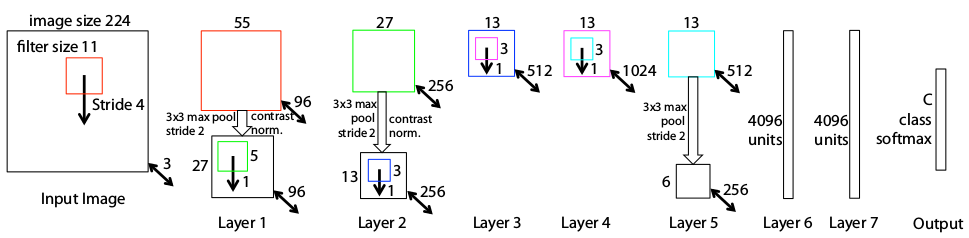
\includegraphics[width=5in]{Figures/arch.png}
	\caption[Res]{Architecture utilise pour le conv net.}
	\label{fig:Electron}
\end{figure}


Le travail s'est basé sur [LeCun et al. 89] et [Kri et al. 12] qu'il a entraîné sur la base d'image de ImageNet 2012 qui contient 1,3 million d'image RGB et 1000 classes. L'Entropie croisée (cross-entropy) fut utilise pour le calcule d'erreur. L’entraînement a été effectué par descente du gradient avec des mini-batch d'une taille de 128 images, un taux d'apprentissage de 0.01 et un dropout sur les dernières couches d'une valeur de 0,5 . Les poids furent initialise à 0.01 et les biais à 0.


[Zei et al. 14] propose dans leur travail une nouvelle manière de retracer les activités des masques de convolution et des caractéristiques qu'ils apprennent vers les pixels qui les ont excite a l'aide de réseaux de déconvolution. Ces derniers reprennent la même architecture que les réseaux a convolution, mais d'une manière inverse. Ils effectuent dans l'ordre suivant: \textbf{Unpooling}: le max-pooling généralement utilise n'est pas inversible. Pour approximer l'inverse de ce dernier l’Idée est donc de sauvegarder l'emplacement du maximum pour chaque région de pooling. Voir figure[]. \textbf{Rectification}: qui s'effectuent a travers l'application de la non linéarité "relu" qui ne fait que prendre le maximum entre la valeur en entrée et 0 pour garder les résultats positifs. Enfin, le \textbf{Filtering}: la dernière étape est d'appliquer les inverses des filtres de convolutions . Ces derniers sont considéré comme étant les transpose des filtres appris. La transpose étant calcule par inversant chaque filtre horizontalement et verticalement.


\begin{figure}[H]
	\centering
		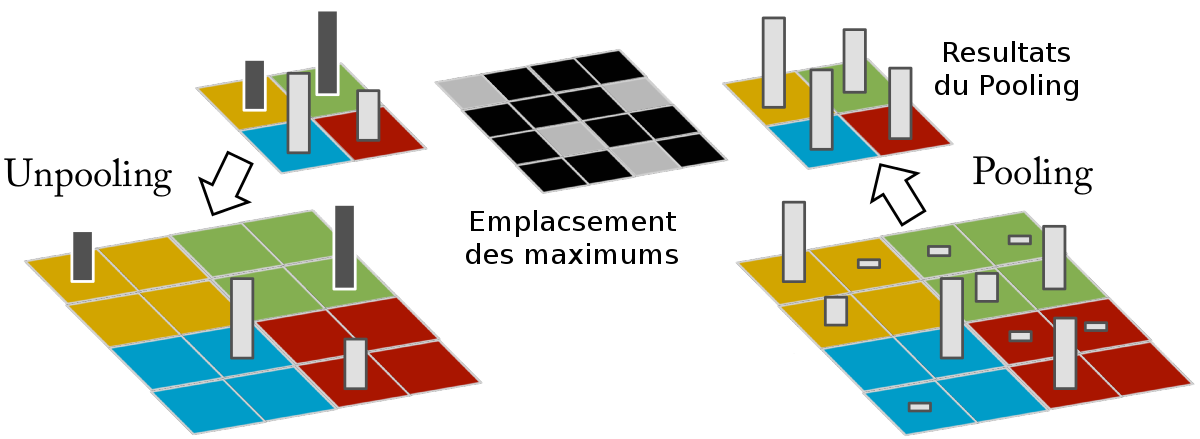
\includegraphics[width=5in]{Figures/unpooling.png}
	\caption[Res]{Chema descriptif du Unpooling.}
	\label{fig:Electron}
\end{figure}

\textbf{Visualisation des caractéristiques}

La tache de visualisation tente de donner un sens a l'apprentissage. Montrer ce que chaque masque détecte peut nous éclaircir sur le sujet. L'approche est donc de tenter de trouver  les zones d'images en entrée qui sont a l'origine de l'activation de chaque masque. 

Par soucis de temps, nous n'avons pas pu implémenter les déconvolutions sur nos modèles. Les résultats obtenu par [Zei et al. 14] sont représenté sur la figure, elle représente le top 9 des zones qui causent le plus grand taux d'activation pour un masque donnée.

On peut voir la nature hiérarchique de la reconnaissance, dans les premières couches, des formes basique sont détecté (la détection de différentes lignes par la couche 1, différents types de coins par la couche 2) et combine d'une couche a une autre pour arriver a des représentations plus complexe (des textures dans la couche 3), jusqu’à pouvoir reconnaître des objets plus significatif dans les dernières couches (humain, chien, roue, fleure ...etc). 

\begin{figure}[H]
	\centering
		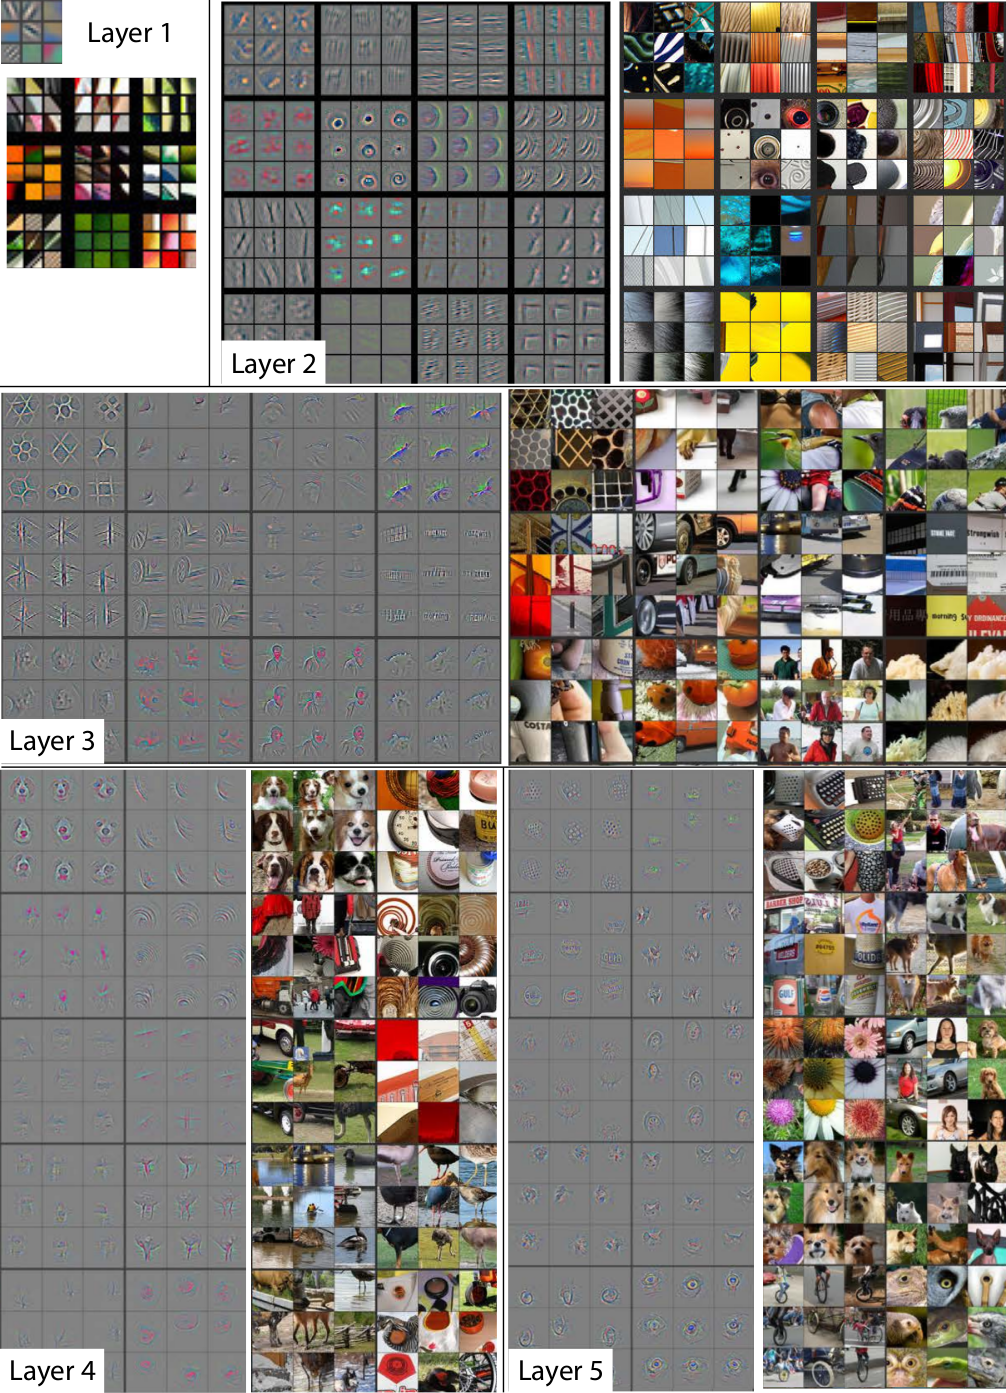
\includegraphics[width=5in]{Figures/visualisation.png}
	\caption[Res]{Visualisation des differentes de l'apprentissage des differentes couches.}
	\label{fig:Electron}
\end{figure}

Mais la aussi, nous savons pas a coup sure si la détection se fait par rapport aux objets, ou a ce qu'ils ont au tour. Pour remédier a ce problème, certaine partie de l'image ont été cachées (avec des rectangles gris), les résultats des testes montrent que le taux de reconnaissance diminue d'une façon radicale, ce qui prouve donc que la détection se fait bien sur les objets eux mêmes.

Nous pouvons donc assumer qu'au final, la représentation retournée par le réseau est bien une représentation sémantique du contenue de l'image qui décris d'une certaine façon son contenue. C'est cette représentation qui sera traduite en termes (1000 libelle des classes) a travers la dernière couche de softmax. Cette représentation force le réseau a utiliser des termes bien précis pour exprimer ce qu'il a appris. C'est de cette raison qu'on retrouve donc de meilleur résultats lors de l'utilisation des sorties de l'avant dernière couche (4000b) ou les concepts appris sont encore libre de cette contrainte. Enfin, plus les représentations sont traites en profondeur, plus elles sont significatifs, et plus le réseau apprend des concepts plus complexes. C'est par ceci que sont expliqués les résultats pas très bons de l'avant avant dernière couche (4000a) (on remarque que les résultats de la couche de softmax (1000) se rapproches de celle de (4000a)).

\subsection{Autoencoder 4x1x4 A REFAIRE} Application d'un réseau d'autoencoder sur les valeurs de la couche 4096b, ce sera un apprentissage qui aura pour but de codifier (convertir) les 4096 valeurs en seulement 1000 valeurs. Ce réseau à une architecture très simple qui est comme suit: 4096 neurones dans la couche d'entrée, 1000 neurones dans la couche cachée et 4096 neurones dans la couche de sortie.
SUPPOSITION: Obtenir de meilleurs résultats que la première approche qui utilise la dernière couche de 1000 neurones par classe.

\begin{figure}[H]
	\centering
		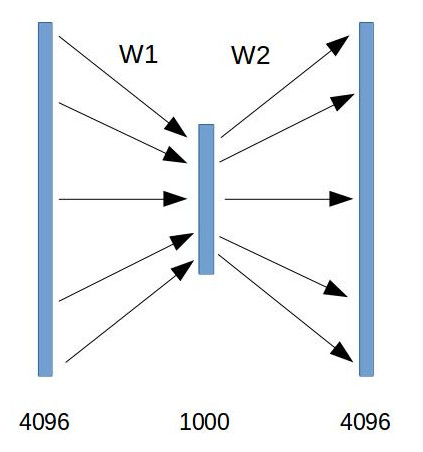
\includegraphics[width=2.5in]{Figures/ae/414.jpg}
	\caption[An Electron]{Architecture Autoencoder 4x1x4.}
	\label{fig:Electron}
\end{figure}

\subsection{Autoencoder 4x2x1x2x4 A REFAIRE} Cette approche utilise une autre architecture d'un réseau autoencoder qui est plus profond que le précédent. Son architecture est comme suit : Une couche d'entrée de 4096 neurones, trois couches cachées ayant dans l'ordre 2000, 1000 et 2000 neurones et finalement la couche de sortie de 4096 neurones.
SUPPOSITION: Obtenir un meilleur taux d'apprentissage que l'autoencoder précedent.

\begin{figure}[H]
	\centering
		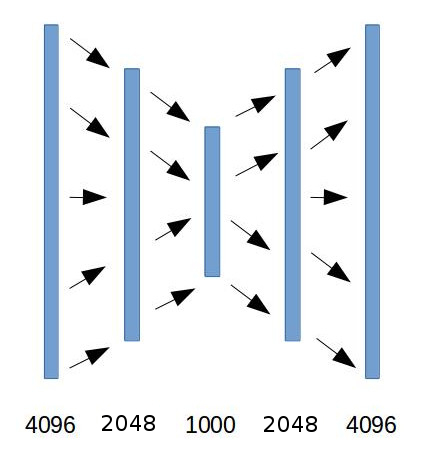
\includegraphics[width=2.5in]{Figures/ae/42124.jpg}
	\caption[An Electron]{Architecture Autoencoder 4x1x4.}
	\label{fig:Electron}
\end{figure}


\subsection{Denoising autoencoder 4x1x4 A REFAIRE} Nous avons tester un autoencoder plus complexe. C'est la même architecture que l'autoencoder 4x1x4, mais avec un taux de corruption de 30\% et moins de paramètre pour éviter au maximum le sur-apprentissage.
SUPPOSITION: Forcer un apprentissage plus significatif et réaliste.

\begin{figure}[H]
	\centering
		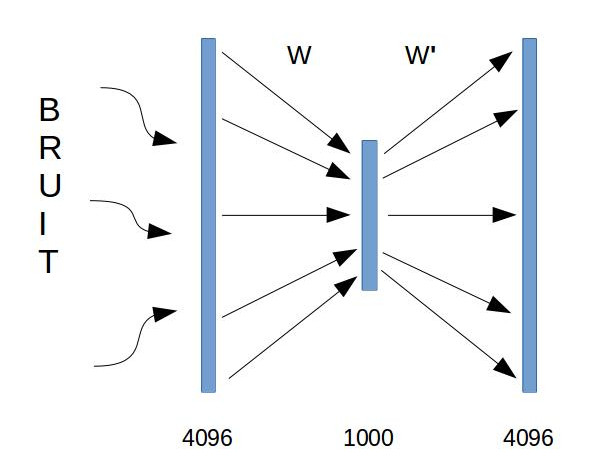
\includegraphics[width=3in]{Figures/ae/denoising.jpg}
	\caption[An Electron]{Architecture Autoencoder 4x1x4.}
	\label{fig:Electron}
\end{figure}

\subsection{Autoencoder 4x1x4 A REFAIRE} avec descripteurs (SIFT,LBP,GLCM,formes,couleurs) : L'architecture de ce réseau ressemble un peu aux précédentes, sauf qu'au lieu de donner en entrée/sortie seulement les 4096 valeurs, on va leurs rajouter différents descripteurs. La combinaison de ses valeurs devra être codifié en 1000 valeurs dans la couche cachée.
 
SUPPOSITION: On ne sait pas si les descripteurs "fabriqués à la main" vont aider à améliorer l'apprentissage ou bien non. Le cerveau n'effectue pas ce genre de calcul, mais l'architecture de l'ordinateur peut lui permettre d'exploiter ses différents descripteurs pour une meilleure reconnaissance.


\begin{figure}[H]
	\centering
		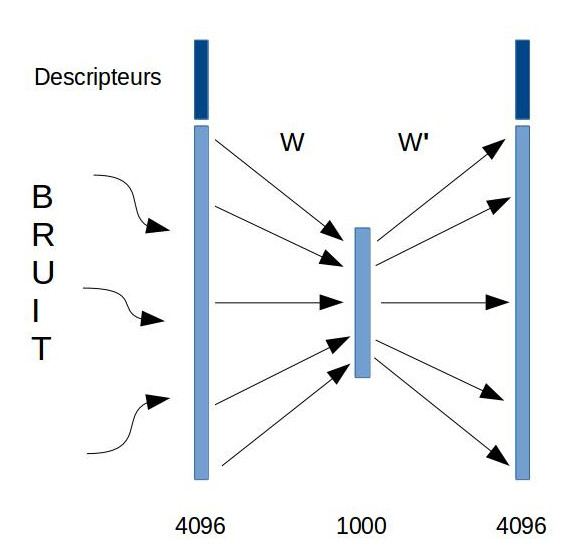
\includegraphics[width=3in]{Figures/ae/AE-Descripteur.jpg}
	\caption[An Electron]{Architecture Autoencoder 4x1x4.}
	\label{fig:Electron}
\end{figure}



\section{EXPLICATION AUTOENCODERS:}
En plus de réduire l'espace de représentation pour prouver que c'est finalement pas ce dernier qui influe sur les résultats, l'utilisation d'auto-encoder ont montré une amelioration considérable des résultats de recherches d'images.

Pour comprendre pourquoi ceci s'est produit nous explorons plus en détails le fonctionnement de l'autoencoder (AE) [Ian et al 2016]. L’idée est, comme expliqué précédemment, dans le chapitre 2, que les données sont concentrées autour d'une partie d'un espace d'une dimension inférieure (appelée Variété ou Manifold) a celle de l'espace de représentation actuelle des données. L'objectif est de retrouver la structure de ce premier. L'AE effectue ceci en faisant le compromis entre deux contraintes (i) Apprendre une représentation \textbf{h} d'un exemple en entrée \textbf{x} (\textbf{h} etant généralement d'une dimensionnalité plus faible) tel que \textbf{x} peut être récupéré a partir de \textbf{h} grâce a un décoder et ce avec un minimum d'erreur. Si \textbf{x} n'appartient pas à l'espace de données en entrée, la reconstruction n'est pas sensée donner de bon résultats. (ii) Le deuxième points à satisfaire est l'ensemble de contraintes de régularisation qui est infligé à l'autoencoder qui ont généralement pour but d’éviter le sur-apprentissage et permettre donc d'avoir une représentation plus générale.


\begin{figure}[H]
	\centering
		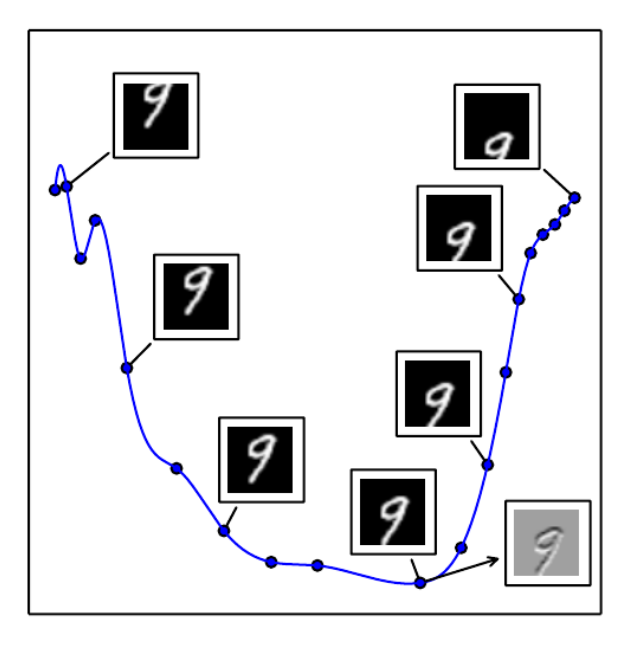
\includegraphics[width=3.5in]{Figures/manifold.png}
	\caption[Res]{Exemple d'une Variété à une dimension dans un espace de 784 dimensions des images de la base MNIST (28×28 pixels). Une image fut prise et déplacée verticalement. Le taux de déplacement vertical défini des coordonnes qui retrace une courbe. Pour la visualiser, cette dernière a été projeté vers un espace 2 dimensions en utilisant PCA (Principal Component Analysis). }
	\label{fig:Electron}
\end{figure}


Nous expliquons donc, dans notre cas, la hausse de niveau de precision par le fait que les représentations sémantiques retenus par le réseau a convolution soient compressé par le "coder", il constitue dorénavant un moyen de résumer les représentations en les combinant d'une façon à en garder ce qu'il y a de plus essentiel.

Ensuite, les contraintes ajouté au Denoising AE lui ont permise d'apprendre une compression plus générale, d’où ses résultats remarquables.

Comparer ces représentations compressées donne donc de meilleurs résultats pour la recherche d'image par contenue.


\section{Conclusion}

Nous concluons ce chapitre en constatant que les méthodes d'apprentissage profond donnent effectivement des résultats très satisfaisants quand on les appliques au problème de recherche d'image par contenue. Même si nos approches pourraient être développé pour donner de meilleur résultats, et en performance, et en temps d’exécution. Nous allons, dans le prochain chapitre, aborder certain détails techniques, mais aussi visualiser concrètement certain résultats de différentes images en requêtes.
%Chapter 4

\chapter{Application} % Main chapter title

\lhead{Chapter 4. \emph{Application}} % This is for the header on each page - perhaps a shortened title


\section{Introduction}
	
	Nous allons aborder dans ce chapitre les détails techniques de notre implémentation (langage de programmation, Frameworks, etc.), ensuite nous présenterons l'interface que nous avons conçu pour l'application de notre approche. Enfin, nous examinerons plus en détail certains exemples et résultats de recherches d'images.

\section{Outils utilisés}

	La configuration de la machine utilisée est comme suit : Processeur Intel R Core TM i7-2670QM CPU @ 2.20GHz , système d’exploitation GNU/Linux - Ubuntu 14.04 x64.

	Nous avons implémenté nos approches avec le langage de programmation Python, version 3.0 et à l'aide de différents Framework et bibliothèques.

	Pour développer l'interface graphique de notre implémentation, nous avons utilisé PyQt4, un module pour python qui permet de le lier à la librairie Qt (framework pour le développement d'applications multi-plate-formes).

\subsection{Le langage Python}
	Nous avons choisi ce langage pour différentes raisons dont nous citons:

\begin{itemize}

\item Une facilité d’écriture et de compréhension du code.
\item Son niveau d'abstraction permet de mettre en place des prototypes et de les tester rapidement
\item Sa syntaxe organisée, l'indentation obligatoire rend le code trivialement lisible.
\item Un grand nombre de bibliothèques puissantes.
\item Une documentation très variée.
\item Une grande communauté qui permet d'obtenir de l'aide rapidement.
\end{itemize}


\subsection{Theano}
	Theano est un framework en Python très utilisé, il est l'un des plus anciens aussi et du coup, beaucoup de recherches se sont basées dessus. 

	Il a été conçu par le laboratoire MILA (Montréal Institute for Learning Algorithms) de l’Université de Montréal. C'est un projet Open Source que de nombreux autre chercheurs de différents laboratoires et institutions ont fini par rejoindre (Google Deepmind, New  York  University, NVIDIA Corporate, Meiji  University Tokyo ..etc ) [Theano 16].

	Ce framework permet de définir des expressions mathématiques symboliques en les représentant par des graphes orientés acycliques. Ces derniers sont constitués de deux types de nœuds: \textbf{Variable} qui représente les données et \textbf{Appliquer} qui représentes les opérations mathématiques. Cette représentation permet une manipulation simple des expressions et fonctions mathématiques dont, entre autre, la génération automatique de leurs dérivées.\\

Par exemple, soit un "scalar" x: \\

>> \textit{x = theano.tensor.dscalar('x')}\\

ensuite on définit une expression, la fonction carré par exemple: \\

>> \textit{y = x ** 2}\\

	On peut aussi visualiser le graphe généré qui résume toute la fonction, avec la ligne suivante:\\

>> \textit{theano.printing.pydotprint(y, outfile="yGraph.png", var\_with\_name\_simple=True)}\\

On aura comme résultat le graphe de la figure [Figure 4.1] ci-dessous:

\begin{figure}[H]
	\centering
		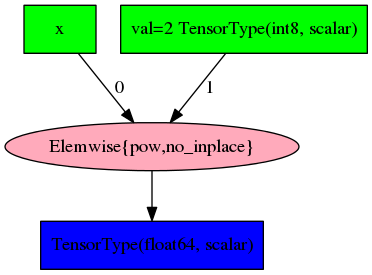
\includegraphics[width=3in]{Figures/yGraph.png}
	\caption[TheanoGraph]{Visualisation du graphe d'une fonction}
	\label{fig:Electron}
\end{figure}

	Les nœuds en verts sont les arguments de l'opérateur puissance (pow) qui est en bleu, et le résultat est dans le nœud en rose.
	Rappelons que lors de la phase d'apprentissage des réseaux de neurones (perceptrons multicouches et autres), il est nécessaire lors de la rétro-propagation du gradient de calculer des dérivés en fonctions de plusieurs paramètres. Theano nous facilite cela puis-que les dérivations s'effectuent simplement en appliquant la fonction \textit{grad}. 
Donc, la dérivée de la fonction \textbf{y} que nous avons définie, par rapport à \textbf{x} peut être calculer comme suit: \\

>> \textit{gy = T.grad(y, x)}\\

\textbf{gy} contient dorénavant la dérivée de \textbf{y} par rapport à \textit{x}, qui n'est rien d'autre que $2*x$ .\\

%>> \textit{theano.pp(gy)}\\
% '((fill((x ** TensorConstant{2}), TensorConstant{1.0}) * TensorConstant{2}) * (x ** (TensorConstant{2} - TensorConstant{1})))'\\
 
	En essayant d'afficher le graphe de \textbf{gy} nous obtenons la figure [Figure 4.2] ci-dessous:

\begin{figure}[H]
	\centering
		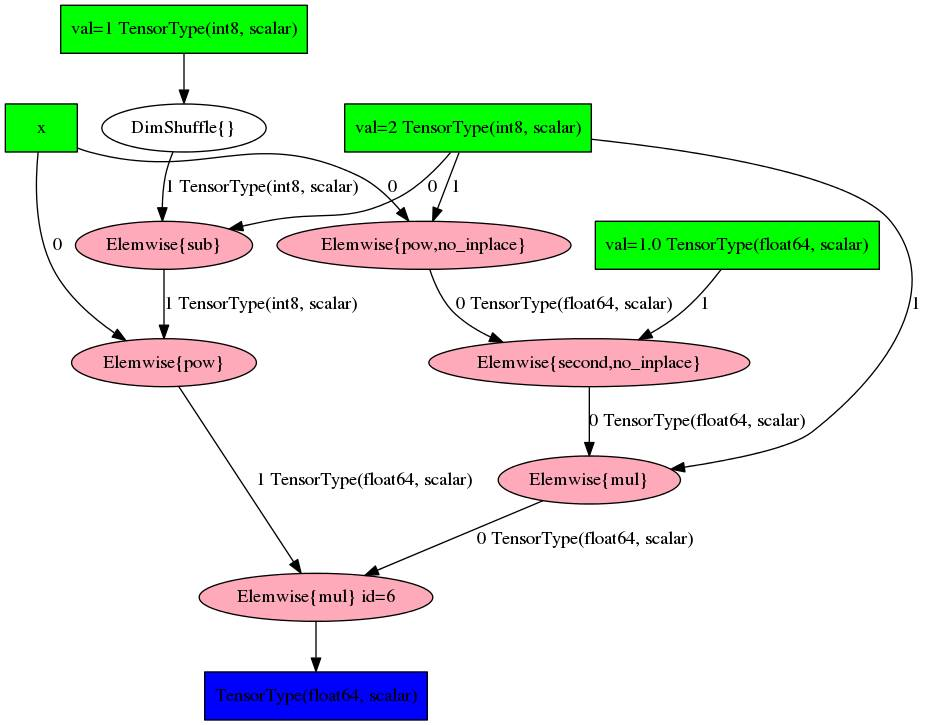
\includegraphics[width=5in]{Figures/beforeOptimization.png}
	\caption[TheanoGraph]{Visualisation du graphe de \textbf{gy} avant optimisation.}
	\label{fig:Electron}
\end{figure}

	Ce graphe n'est pas évident à comprendre alors qu'il s'agit seulement de la fonction $ gy = 2*x$. Compiler le graphe de \textbf{gy} à l'aide de la fonction "function" de Theano pour le rendre exécutable s'effectue comme suit:\\

>> \textit{f = theano.function([x], gy)}\\

	Cette opération optimise le calcul de \textbf{gy}, et le graphe de \textbf{f} devient comme le montre la figure ci-dessous:

\begin{figure}[H]
	\centering
		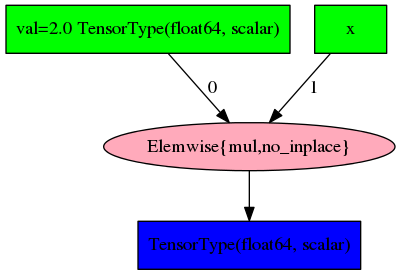
\includegraphics[width=3in]{Figures/afterOptimization.png}
	\caption[TheanoGraph]{Visualisation du graphe de \textbf{gy} après optimisation.}
	\label{fig:Electron}
\end{figure}

	Ceci montre à quel point Theano est puissant dans sa gestion des fonctions et de leurs dérivées, ainsi que leurs optimisations en quelques lignes de codes.
	
	Une notion très importante qui existe dans Theano est celle des \textit{variables symboliques}. Elle peuvent être considérées comme des tampons (buffers) qui contiennent des valeurs qui peuvent être partagées entre plusieurs fonctions de Theano.\\

	Un autre point fort de Theano est l'optimisation pour l'utilisation de matrices multi-dimensionnelles, mais aussi la facilité de compiler et exécuter les opérations sur des GPU au lieu des CPU.\\

	Theano fut suivi par d'autres frameworks qui ont repris les mêmes principes, les plus connus sont Tensorflow de Google, Blocks, Lasagne.

\subsection{Autres Frameworks}
	Pour ce familiariser avec Theano, il existe d'autres frameworks qui ajoutent des couches d'abstraction à Theano pour faciliter son utilisation, comme Blocks, Lasagne et Keras.
	Le modèle VGG-CNN-S du réseau à convolution que nous avons utilisé dans notre algorithme est implémenté en Lasagne après avoir été converti de Caffe (Caffe étant un autre Framework en C++ développé par le laboratoire Berkeley Vision and Learning Center).\\

	Pour implémenter les autoencoders de nos approches, nous avons utilisé Blocks [Mer et al. 15], c'est un framework de theano qui facilite la définition de modèles et leur modifications. Il introduit des outils pour l'apprentissage, la visualisation et la sérialisation. Enfin, le framework Fuel [Mer et al. 15] permet de formater les données d'apprentissage d'une façon qui facilite leur manipulation, surtout quand les tailles de ces dernières deviennent importantes.\\

	Dans notre cas, au lieu de le définir couche par couche, l'Autoencoder 4x1x4 est défini simplement par:\\

>> \textit{ae = MLP([Tanh(), Tanh()], [4096, 1000, 4096],
              weights\_init=IsotropicGaussian(0.01),
              biases\_init=Constant(0))\\
   }           

Puis, il est initialisé par:\\

>> ae.initialize()\\

	Ces deux frameworks sont développés aussi par le laboratoire MILA, ils forment une base solide pour le développement d’approches basées sur l'apprentissage profond.

\section{Interface de l'application}

	Après notre étude comparative dans le chapitre précédent entre les différentes approches que nous avons réalisées, nous avons décidé d'implémenter dans l'interface graphique la meilleure approche (celle qui a donné les meilleures mesures de performance), qui est celle du Denoising Autoencoder 4x1x4.

	L'interface que nous avons développée [Figure 4.2] pour l'implémentation de notre approche permet de sélectionner une base d'images qui servira de recueil pour les résultats des requêtes, comme le montre la figure ci dessous:


\begin{figure}[H]
	\centering
		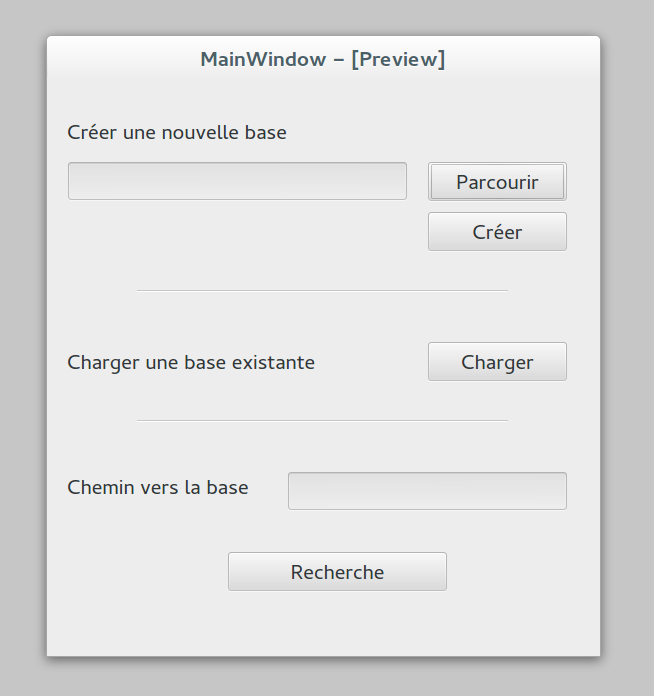
\includegraphics[width=3in]{Figures/mainMenu.png}
	\caption[Menu principal]{Menu principal}
	\label{fig:Electron}
\end{figure}

	Nous pouvons choisir de créer une nouvelle base, pour cela on doit indiquer le lien vers le dossier contenant la base d'images, puis appuyer sur le bouton \textit{Créer}. Le programme dans ce cas va créer la description de chaque image en la faisant passer par le réseau à convolution, ensuite extraire la description sémantique de l'image de la couche 4096b et finalement créer la description compressée en utilisant le Denoising Autoencoder 4x1x4.
	C'est cette description qui sera enregistrée en tant que modèle pour la recherche d'images. On peut aussi charger une base déjà existante en appuyant sur le bouton \textit{Charger}.

	En cliquant sur le bouton "Recherche", une nouvelle fenêtre s'ouvre qui permet de sélectionner une image qui fera office de requête [Figure 4.3]. Une fois l'image sélectionnée, le programme va créer sa représentation sémantique compressée. Le bouton "Chercher" lance la recherche et affiche les cinq images jugées les plus ressemblantes (top-5).

\begin{figure}[H]
	\centering
		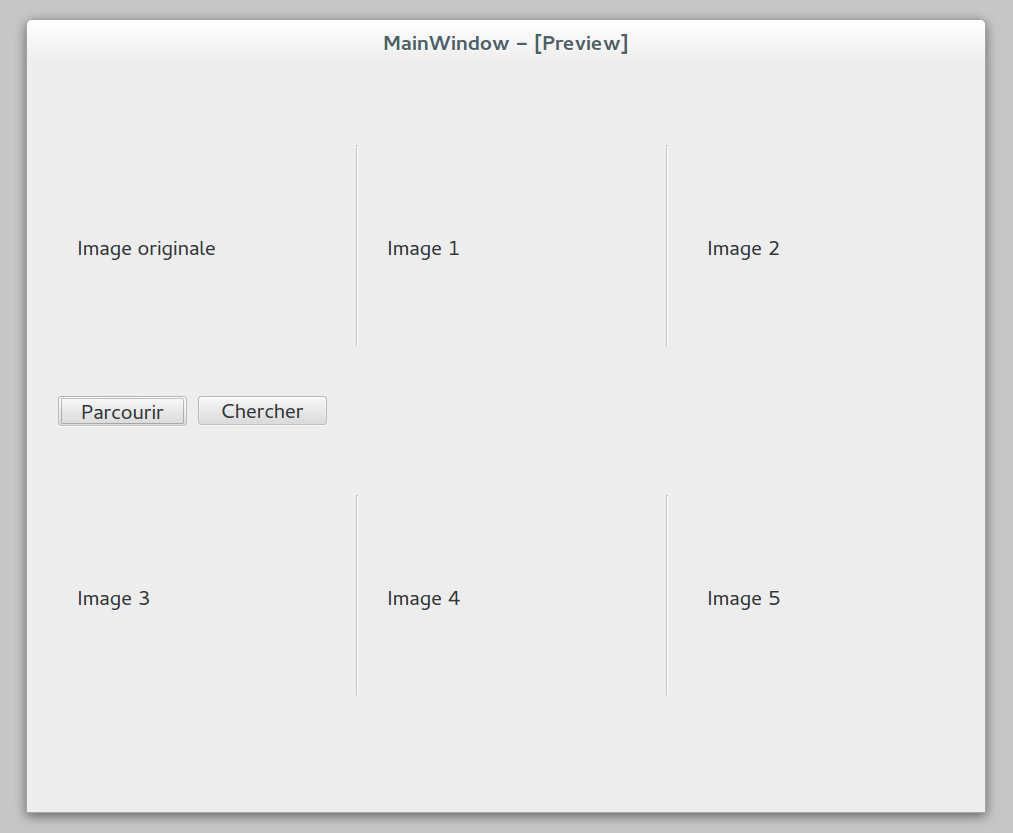
\includegraphics[width=5in]{Figures/search.png}
	\caption[]{Interface de recherche d'images.}
	\label{fig:Electron}
\end{figure}

\section{Tests}

La figure A et B ci-dessous représente deux testes effectués sur deux images tirées respectivement des bases \textbf{Wang} et \textbf{Caltech}. Nous pouvons bien voir la qualité des résultats obtenus sur le top 5 des images retournées.

\begin{figure}[H]
	\centering
		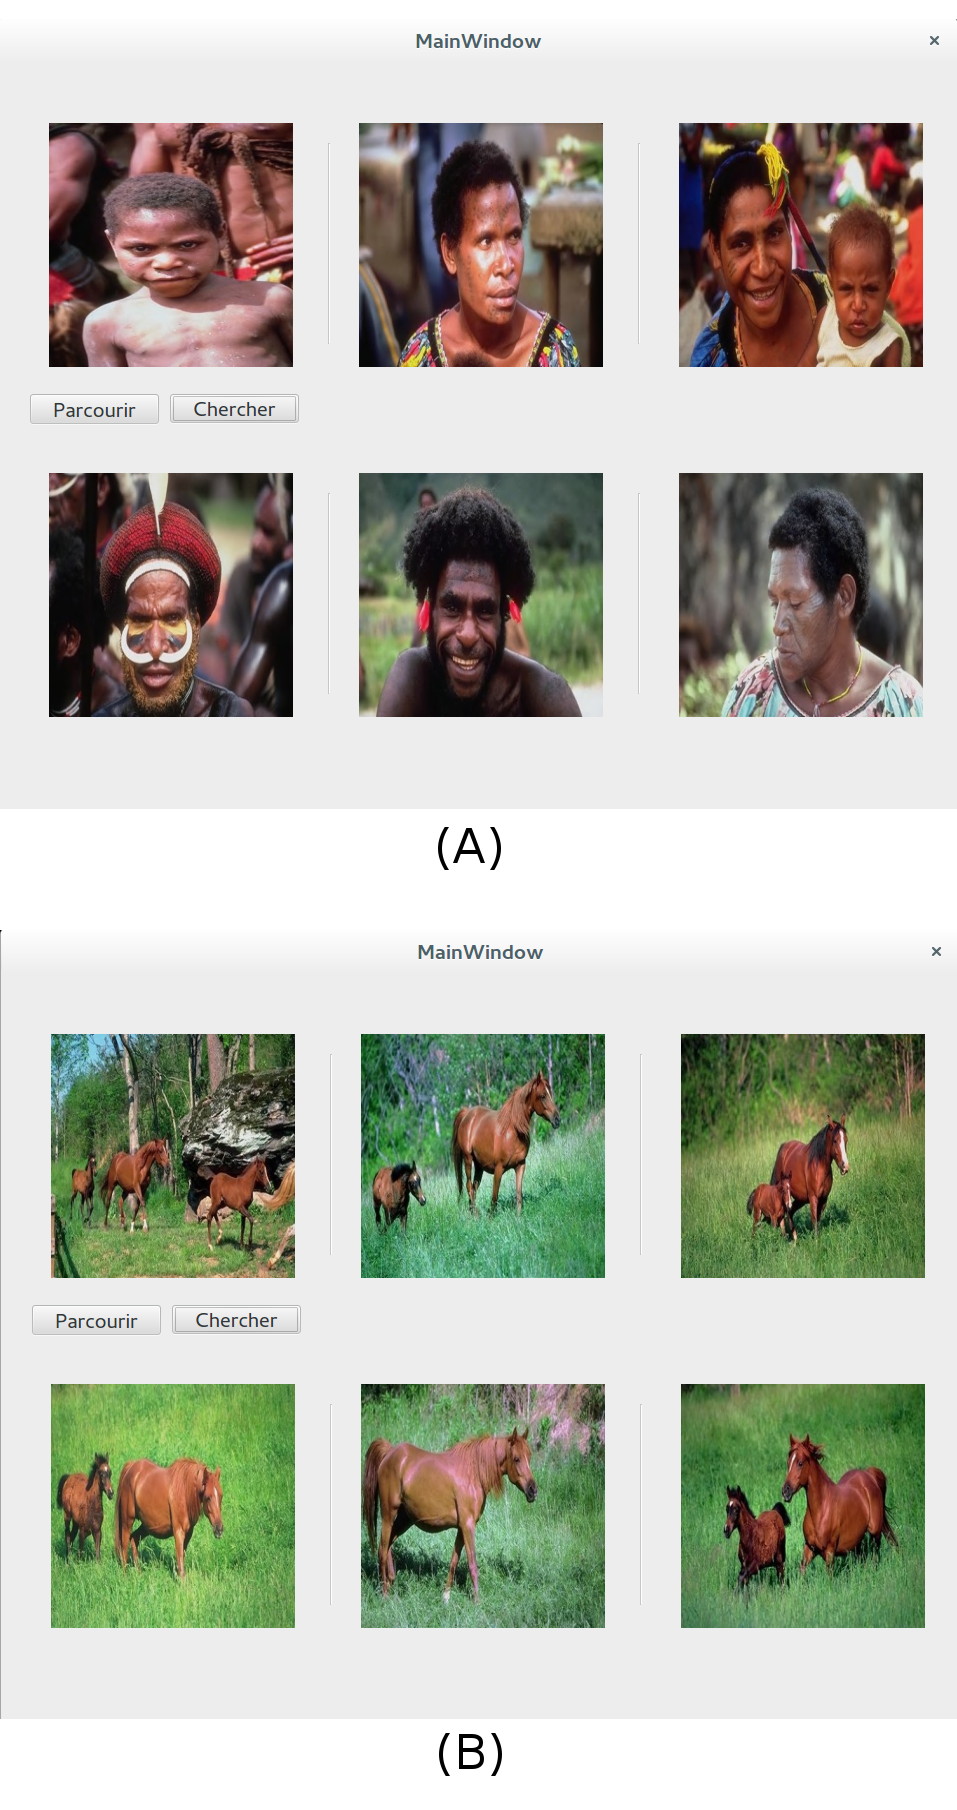
\includegraphics[width=4in]{Figures/guiTests.png}
	\caption[]{Test sur deux images respectivement des bases \textbf{Wang} et \textbf{Caltech}.}
	\label{fig:Electron}
\end{figure}


\section{Conclusion}

Nous concluons ce chapitre en mettant le point sur les avantages qu'apporte de la représentation symbolique derrière le framework Theano. Ceci permet entre autre de faciliter la description de modèles complexes mais aussi de faciliter leur entraînement (en retro-propagation) grâce au calcule automatique des dérivés. Nous avons aussi montré des résultats sur différents exemples de requêtes ou nous avons pu observer en détail... 
%Chapter 5

\chapter*{Conclusion générale} % Main chapter title

Nous avons, durant notre travail, fait une recherche approfondie sur les techniques d'intelligence artificielle utilisées par les plus grands laboratoires de recherches dans le monde entier (Facebook AI Reaserch, Google DeepMind, Montréal Institute for Learning Algorithms et d'autre), et plus spécialement celles qui sont appliquées dans le domaine du traitement d'image. C'est ainsi que nous avons découvert cette nouvelle tendance qui est l'apprentissage profond (Deep Learning), vers laquelle pratiquement toutes les recherches scientifiques qui traitent de grandes masses de données essayent d'exporter leur recherche. Ceci étant dû à la puissance de ses techniques et aux résultats phénoménaux qu'elles continuent à produire, et qui semblent facilement surpasser les techniques classiques.

	De notre part, nous avons proposé des approches dans le problème de recherche d'image par le contenu (CBIR) où nous avons essayé, dans ce travail, de faire apprendre à la machine à créer des représentations sémantiques d'une image, dans le but de pouvoir la comparer avec d'autres images.

	Nous avons essayé différentes approches, et avons démontré que la différence de précision entre les couches des réseaux à convolutions, n’était pas dû à la compression des espaces de représentation (de 4096 valeurs à seulement 1000 valeurs) mais plutôt au type de l'information que contiennent les représentations, et à quelle profondeur le traitement se fait. 

Nous avons aussi montré que l'ajout de certains descripteurs fabriqués à la main (description de texture, couleur, forme) n'avait finalement pas autant d'impact sur les descriptions sémantiques des réseaux à convolutions. Cela est logique, car il est très peu probable que le cerveau humain effectue ce genre d’opérations mathématiques formelles. Comme l'apprentissage profond tente d'imiter le fonctionnement du cerveau, ces descripteurs traditionnels s’avéreront très peu utiles.

Une amélioration de la structure de nos descriptions et du temps de recherche peut-être permise grâce à l'apprentissage d'une représentation binaire, au lieu d'une représentation par une liste de nombres réels. Elle permettrait la construction d'un arbre de hachage qui optimisera le temps de recherche et de récupération d'images similaires. Une méthode inspiré par le travail de [Kri et al. 11] qui ont fait passé leurs images (représentations en pixels) dans un autoencoder à base de réseau de croyances (DBN), et les ont compressé en une représentation binaire. Nous pensons qu'une approche similaire mais qui prendrait, au lieu des pixels brutes de l'image, l'information sémantique apprise par le réseau à convolution pourrait donner de meilleurs résultats.

	
%Essayer d'autres mesures de distance

 


%\bibliographystyle{unsrt}%introduire les references plain | alpha unsrt apalike-fr
%\bibliography{biblio}
%\addcontentsline{toc}{chapter}{Bibliographie }
%\addcontentsline{toc}{chapter}{Annexe}
%\appendix
\end{spacing}
\end{document}